% =====================================================================
%  diatomic-chain  ·  Technical documentation (English)
%  Author: Jesús García Izquierdo
%  Repository: https://github.com/jesus-garcia-izquierdo/diatomic-chain
%  Build with:  xelatex diatomic_chain_en.tex  (run twice)
% =====================================================================
\documentclass[11pt,a4paper]{article}

\usepackage{fontspec}
\usepackage{polyglossia}
\setdefaultlanguage[variant=british]{english}
\setmainfont{Latin Modern Roman}
\setsansfont{Latin Modern Sans}
\setmonofont{Latin Modern Mono}

\usepackage{amsmath,amssymb,mathtools,bm}
\usepackage[margin=2.4cm]{geometry}
\usepackage{graphicx}
\graphicspath{{../figures/}}
\usepackage{booktabs,array,tabularx}
\usepackage[dvipsnames]{xcolor}
\usepackage{enumitem}
\usepackage[font=small,labelfont=bf]{caption}
\usepackage[most]{tcolorbox}
\usepackage{hyperref}
\hypersetup{colorlinks=true,linkcolor=NavyBlue,citecolor=NavyBlue,urlcolor=NavyBlue,
  pdftitle={Jesús García Izquierdo - https://github.com/jesus-garcia-izquierdo/diatomic-chain | diatomic-chain: diatomic chain, phonons and heat capacity},
  pdfauthor={Jesús García Izquierdo}}

% ---------- Colours of the five elements (terminology of the Mechanics notes)
\definecolor{eobj}{HTML}{2a78d6}
\definecolor{ecam}{HTML}{eb6834}
\definecolor{eaco}{HTML}{1baf7a}
\definecolor{eesc}{HTML}{6250d6}
\definecolor{eobs}{HTML}{e34948}
\newcommand{\Eobj}{object\textsuperscript{\textcolor{eobj}{\textbf{E1}}}}
\newcommand{\Ecam}{field\textsuperscript{\textcolor{ecam}{\textbf{E2}}}}
\newcommand{\Ecams}{fields\textsuperscript{\textcolor{ecam}{\textbf{E2}}}}
\newcommand{\Eaco}{coupling\textsuperscript{\textcolor{eaco}{\textbf{E3}}}}
\newcommand{\Eesc}{stage\textsuperscript{\textcolor{eesc}{\textbf{E4}}}}
\newcommand{\Eobs}{observer\textsuperscript{\textcolor{eobs}{\textbf{E5}}}}

% ---------- Boxes
\newtcolorbox{idea}[1][Key idea]{colback=NavyBlue!4,colframe=NavyBlue!70,
  fonttitle=\bfseries\small,title=#1,boxrule=0.6pt,arc=2pt,left=6pt,right=6pt}
\newtcolorbox{codigo}[1][In the code]{colback=ForestGreen!4,colframe=ForestGreen!65,
  fonttitle=\bfseries\small,title=#1,boxrule=0.5pt,arc=2pt,left=6pt,right=6pt}

% ---------- Macros
\newcommand{\kB}{k_{\mathrm B}}
\newcommand{\dd}{\mathrm{d}}
\newcommand{\ii}{\mathrm{i}}
\newcommand{\ee}{\mathrm{e}}
\newcommand{\avg}[1]{\left\langle #1\right\rangle}
\newcommand{\vs}{v_{s}}
\newcommand{\code}[1]{\texttt{#1}}

\setlist{itemsep=2pt,topsep=4pt}
\setlength{\parskip}{3pt}
\setlength{\emergencystretch}{3em}
\tolerance=1500

\begin{document}

% =====================================================================
\begin{titlepage}
\centering
\vspace*{2.2cm}
% Título obligatorio (H1): "Jesús García Izquierdo - https://github.com/jesus-garcia-izquierdo/diatomic-chain"
{\LARGE\bfseries Jesús García Izquierdo -\par}
\vspace{6pt}
{\Large\bfseries\mbox{\href{https://github.com/jesus-garcia-izquierdo/diatomic-chain}{https://github.com/jesus-garcia-izquierdo/diatomic-chain}}\par}
\vspace{1.6cm}
\rule{0.75\textwidth}{0.6pt}\par\vspace{0.5cm}
{\Large Diatomic chain: acoustic and optical branches,\\[2pt]
phonon density of states and heat capacity\par}
\vspace{0.3cm}
{\large Numerical heat capacity versus the Debye and Einstein models,\\
displacement fluctuations and validation by Langevin dynamics\par}
\vspace{0.5cm}
\rule{0.75\textwidth}{0.6pt}\par
\vspace{1.4cm}
{\large Technical and theoretical documentation (English version)\par}
\vspace{0.3cm}
{\normalsize MSc in Condensed Matter Physics\par}
\vfill
{\normalsize October 2026\par}
\end{titlepage}

% =====================================================================
\begin{abstract}
\noindent
This document collects the theory and the results of the
\texttt{diatomic-chain} repository. The presentation goes \emph{from the most
general to the most particular}: we start from the description of a solid as a
mechanical problem (the five elements: \Eobj, \Ecams, \Eaco, \Eesc{} and
\Eobs), arrive at the harmonic crystal and its statistical-mechanical
description in the canonical ensemble as an \emph{ideal} system of oscillators
(phonons), introduce the density of states (DOS) and the Einstein and Debye
models, and only then specialise to the one-dimensional diatomic chain with two
masses $m_1,m_2$ and, in general, two spring constants $K_1,K_2$. For it we
obtain in closed form the acoustic and optical branches, the DOS and the
cumulative number of modes; we compute numerically (Gauss–Legendre quadrature
over the Brillouin zone) the heat capacity, internal energy, entropy and free
energy; and we compare them quantitatively with the Debye model, the Einstein
model and a hybrid Debye\,+\,Einstein model. We also discuss other observables:
the effective Debye temperature $\Theta_D(T)$, the fluctuations of the atomic
displacements (absence of long-range positional order in 1D) and bond
fluctuations. Everything is validated along an independent route: a Langevin
dynamics simulation (BAOAB integrator) from which we extract the DOS (velocity
spectrum), the heat capacity (fluctuation–response relation) and the
displacement correlations.
\end{abstract}

\tableofcontents
\newpage

% =====================================================================
\section*{Notation and units}
\addcontentsline{toc}{section}{Notation and units}

Unless stated otherwise we work in \textbf{reduced units} $\hbar=\kB=1$, so an
angular frequency, an energy and a temperature are measured in the same unit;
the natural scale is $\sqrt{K/m_1}$. To convert to physical units recall that
typical phonon energies are $\hbar\omega\sim 10$–$100$\,meV, i.e.\
characteristic temperatures $\Theta=\hbar\omega/\kB\sim 10^2$–$10^3$\,K.

\begin{center}
\small
\begin{tabularx}{\textwidth}{@{}l X@{}}
\toprule
Symbol & Meaning \\
\midrule
$m_1,\ m_2$ & masses of the two atoms of the basis (sublattices $s=1,2$)\\
$K_1,\ K_2$ & spring constants of the intra-cell and inter-cell bonds\\
$a$ & lattice constant (length of the two-atom unit cell)\\
$N$ & number of cells; $2N$ atoms and $2N$ normal modes\\
$\sigma=K_1+K_2$,\ $\mu=m_1m_2/(m_1+m_2)$,\ $M=m_1+m_2$ & sum of spring constants, reduced mass, cell mass\\
$u_{s,n}$ & displacement of atom $s$ of cell $n$ from its equilibrium position\\
$k$ & wave number in the first Brillouin zone $(-\pi/a,\pi/a]$\\
$\omega_-(k),\ \omega_+(k)$ & acoustic and optical branches\\
$\vs$ & sound velocity, $\vs=a\sqrt{K_1K_2/[(K_1+K_2)M]}$\\
$g(\omega)$ & phonon DOS per cell, $\int_0^\infty g\,\dd\omega=2$\\
$N(\omega)$ & cumulative number of modes per cell, $N(\omega)=\int_0^\omega g$\\
$\beta=1/\kB T$ & inverse thermal energy of the bath\\
$C_V$ & heat capacity at fixed external parameters (here, fixed length)\\
$\Theta_D,\ \Theta_E$ & Debye and Einstein temperatures\\
\bottomrule
\end{tabularx}
\end{center}

% =====================================================================
\part*{Part I. General framework}
\addcontentsline{toc}{part}{Part I. General framework}
% =====================================================================

\section{What we describe and with which ingredients}

\subsection{State, observables and dynamics}

Every mechanical theory answers three questions: \emph{what} information is
enough to specify the system now (\textbf{state}), \emph{which} quantities can
be measured (\textbf{observables}) and \emph{how} the state changes in time
(\textbf{dynamics}). A crystalline solid has about $10^{23}$ degrees of
freedom, so the complete microscopic description (a point of classical phase
space, or a quantum state vector) is unmanageable and irrelevant for
macroscopic purposes. Statistical mechanics replaces the microstate by a
\emph{macrostate} $\mathcal B$ characterised by a probability distribution over
microstates (the ensemble), and the macroscopic values of the observables are
averages over it. This project is a particularly clean example of that
programme, because in the harmonic approximation the microscopic dynamics is
solved \emph{exactly} and the statistics reduce to those of an ideal system.

\subsection{The five elements applied to a solid}

Before writing any equation it pays to separate the five elements of the
physical problem: an \Eobj{} (what moves), some \Ecams{} (what acts on it), a
\Eaco{} (how they act), a \Eesc{} (the background structure, with its
symmetries) and an \Eobs{} (the choice of variables and approximations used to
read the problem). Much conceptual confusion comes from mixing them.

\begin{center}
\small
\begin{tabularx}{\textwidth}{@{}l X@{}}
\toprule
Element & In a crystal (and in the diatomic chain)\\
\midrule
\Eobj & The nuclei (with their core electrons) of masses $m_s$; state variables: displacements $u$ and momenta $p$.\\
\Ecams & The effective potential $V(\{\bm R\})$ created for the nuclei by the valence electrons in the Born–Oppenheimer approximation.\\
\Eaco & The forces $-\partial V/\partial \bm R$; in the harmonic approximation, linear springs $K_1,K_2$ between nearest neighbours.\\
\Eesc & The Bravais lattice with a two-atom basis: \emph{discrete translation} symmetry by multiples of $a$.\\
\Eobs & Chosen representation: atomic displacements, normal coordinates, Bloch waves $|k\rangle$ or phonon occupation numbers.\\
\bottomrule
\end{tabularx}
\end{center}

The moral that guides the whole document is the chain
\[
\text{\Eesc}\ \Longrightarrow\ \text{symmetries}\ \Longrightarrow\ \text{conserved quantities and good quantum numbers}.
\]
In the crystal, the discrete translation symmetry of the \Eesc{} turns the
wave number $k$ (the \emph{crystal momentum}) into a good quantum number and
lets us diagonalise the problem block by block (Bloch's theorem).

\subsection{System and environment: the crystal in contact with a bath}

A real crystal is never isolated: it exchanges energy with its environment. We
model it as a \emph{closed system} in contact with a much larger heat bath, with
a weak coupling whose only role is to allow heat exchange. Once equilibrium is
reached the macrostate is $\mathcal B=(\beta,N,L)$ and the distribution of
microstates is the \textbf{canonical} one,
\begin{equation}
\rho_{\mathcal B}\propto \ee^{-\beta \hat H}, \qquad
Z(\beta)=\operatorname{tr}\ee^{-\beta\hat H},\qquad
F=-\beta^{-1}\ln Z .
\end{equation}
From $Z$ follow the macroscopic values:
\begin{equation}
\avg{E}=-\frac{\partial \ln Z}{\partial\beta},\qquad
C_V=\kB\beta^2\frac{\partial^2\ln Z}{\partial\beta^2},\qquad
S=\frac{\avg{E}-F}{T}.
\end{equation}
In the thermodynamic limit the microcanonical and canonical ensembles coincide
and the relative energy fluctuation vanishes (\S\ref{sec:fluct}).

% =====================================================================
\section{From the real solid to the harmonic crystal}

\subsection{Equilibrium configuration and expansion of the potential}

The first step is static: the equilibrium configuration $\{\bm R^0\}$ makes
the forces vanish, $\partial V/\partial\bm R=0$. Writing $\bm R=\bm R^0+\bm u$
and expanding,
\begin{equation}
V = V_0 + \frac12\sum_{i,j}\Phi_{ij}\,u_iu_j + \mathcal O(u^3),
\qquad \Phi_{ij}=\left.\frac{\partial^2V}{\partial u_i\,\partial u_j}\right|_0 .
\end{equation}
The \textbf{force-constant matrix} $\Phi$ is symmetric and, if the equilibrium is
stable, positive semidefinite. Invariance of the \Eesc{} under rigid
translations imposes the \emph{acoustic sum rule} $\sum_j\Phi_{ij}=0$: moving
the whole crystal costs no energy.

\subsection{Small oscillations and normal coordinates}\label{sec:normales}

With $T=\tfrac12\sum_i m_i\dot u_i^2$ Newton's equations read
$M\ddot{\bm u}=-\Phi\bm u$ with $M=\operatorname{diag}(m_i)$. Looking for
solutions $\bm u\propto\bm v\,\ee^{-\ii\omega t}$ leads to the generalised
eigenvalue problem
\begin{equation}
\boxed{\det\!\left(\Phi-\omega^2 M\right)=0}
\label{eq:secular}
\end{equation}
which is the same mathematics that reappears with quantum observables:
diagonalising a Hermitian operator. It is convenient to symmetrise it with the
\textbf{dynamical matrix} $D=M^{-1/2}\Phi M^{-1/2}$, Hermitian and positive
semidefinite, whose eigenvalues are $\omega^2\geq0$ and whose orthonormal
eigenvectors $\bm e_\lambda$ define the \textbf{normal coordinates}
$Q_\lambda$. In them
\begin{equation}
H=\sum_\lambda\left(\frac{P_\lambda^2}{2}+\frac{\omega_\lambda^2Q_\lambda^2}{2}\right),
\end{equation}
i.e.\ the harmonic crystal is an \textbf{ideal system}: a collection of
\emph{decoupled}, \emph{distinguishable} oscillators. All the physics of the
interactions is hidden in the spectrum $\{\omega_\lambda\}$.

\begin{idea}
Anharmonicity ($\mathcal O(u^3)$) is the \emph{residual interaction} of this
ideal system. Energetically it is small, but conceptually it is essential:
without it each normal mode would keep its energy forever, the dynamics would be
integrable and an isolated realisation of the crystal would \emph{not} be
ergodic nor mixing (the famous Fermi–Pasta–Ulam–Tsingou experiment shows that a
weak anharmonicity is not always enough either). In the canonical ensemble this
is no problem: the heat bath thermalises each mode separately. In the simulation
of \S\ref{sec:langevin} the Langevin bath plays exactly that role.
\end{idea}

\subsection{Discrete translation symmetry: Bloch's theorem}

For a crystal of $N$ cells with $p$ atoms per cell in $d$ dimensions, $D$ has
dimension $dpN$. Discrete translation symmetry lets us look for Bloch-wave
solutions,
\begin{equation}
u_{s,n}(t)=\frac{e_s}{\sqrt{m_s}}\,\ee^{\ii(kna-\omega t)},
\end{equation}
which reduce the problem to a $dp\times dp$ matrix $D(k)$ for each $k$ in the
first Brillouin zone. With Born–von Kármán periodic boundary conditions,
$u_{s,n+N}=u_{s,n}$, the allowed wave numbers are
\begin{equation}
k_j=\frac{2\pi j}{Na},\qquad j=-\tfrac N2+1,\dots,\tfrac N2,
\end{equation}
exactly $N$ values. For each $k$ there are $dp$ frequencies $\omega_b(k)$:
the \textbf{branches} of the dispersion relation.
\begin{itemize}
\item $d$ \textbf{acoustic} branches, with $\omega\to0$ as $k\to0$: they are the
  manifestation of the acoustic sum rule (Goldstone modes of the translation
  symmetry broken by the crystal). At long wavelength they are sound waves,
  $\omega\simeq \vs|k|$.
\item $d(p-1)$ \textbf{optical} branches, with $\omega(0)\neq0$: the atoms of
  the basis oscillate against each other. If they carry different charges,
  these modes couple to light (hence the name).
\end{itemize}
In total there are $dpN$ modes, as many as degrees of freedom.

% =====================================================================
\section{Statistical mechanics of the harmonic crystal}

\subsection{Quantisation: phonons}

Quantising each normal oscillator,
\begin{equation}
\hat H=\sum_{k,b}\hbar\omega_b(k)\left(\hat n_{k,b}+\tfrac12\right),
\qquad \hat n_{k,b}=0,1,2,\dots
\end{equation}
The excitation number $n_{k,b}$ is interpreted as the number of
\textbf{phonons} in mode $(k,b)$. Phonons are bosons whose number is
\emph{not conserved} (the bath can freely create and destroy them), so their
chemical potential vanishes and their mean number follows Bose–Einstein
statistics with $\mu=0$:
\begin{equation}
\avg{n}=\frac{1}{\ee^{\beta\hbar\omega}-1}.
\end{equation}

\subsection{Canonical ensemble: everything factorises}

Being an ideal system of distinguishable oscillators, the partition function
factorises,
\begin{equation}
Z(\beta)=\prod_{k,b}\frac{1}{2\sinh\!\left(\beta\hbar\omega_b(k)/2\right)},
\qquad
\ln Z=-\sum_{k,b}\ln\!\left[2\sinh\!\left(\tfrac{\beta\hbar\omega_b(k)}{2}\right)\right],
\end{equation}
and any macroscopic quantity is a sum of single-mode contributions. With
$y=\hbar\omega/\kB T$, the single-oscillator functions are:

\begin{center}
\small
\begin{tabular}{@{}lll@{}}
\toprule
Quantity & Quantum & Classical ($y\to0$)\\
\midrule
mean energy & $e=\dfrac{\hbar\omega}{2}\coth\dfrac y2=\dfrac{\hbar\omega}{2}+\hbar\omega\avg{n}$ & $\kB T$\\[6pt]
heat capacity & $c=\kB\,\dfrac{(y/2)^2}{\sinh^2(y/2)}$ & $\kB$\\[6pt]
free energy & $f=\kB T\ln\!\left[2\sinh(y/2)\right]$ & $\kB T\ln y$\\[4pt]
entropy & $s/\kB=y\avg{n}-\ln(1-\ee^{-y})$ & $1-\ln y$\\
\bottomrule
\end{tabular}
\end{center}

\noindent $c(y)$ is the \emph{Einstein function}. Two limits summarise it. If
$T\gg\Theta_{\rm vib}=\hbar\omega/\kB$ the oscillator is classical and
contributes $\kB$ (equipartition theorem: $\kB/2$ per quadratic term of the
Hamiltonian). If $T\ll\Theta_{\rm vib}/10$ the oscillator is almost always in
its ground state: it is \textbf{frozen} and does not contribute to the heat
capacity. The whole phenomenology of the heat capacity of solids can be read as
the progressive ``unfreezing'' of the modes as temperature rises.

Summing over the $dpN$ modes, the classical limit gives the \textbf{Dulong–Petit
law}: $C_V=dpN\kB$, independent of masses and spring constants. In our chain
($d=1$, $p=2$): $C_V/N\kB\to2$, i.e.\ $\kB$ per atom.

\subsection{Phonon density of states}

When $N\to\infty$ the $k$ values form a continuum. The continuum limit
$\frac1N\sum_k\to\frac{a}{2\pi}\int_{\rm BZ}\dd k$ turns sums over modes into
integrals, and it is convenient to group modes by frequency through the
\textbf{density of states} (DOS) per cell:
\begin{equation}
g(\omega)=\frac1N\sum_{k,b}\delta\!\left(\omega-\omega_b(k)\right)
=\frac{a}{2\pi}\sum_b\int_{\rm BZ}\dd k\;\delta\!\left(\omega-\omega_b(k)\right),
\qquad \int_0^\infty g(\omega)\,\dd\omega = dp .
\end{equation}
With it, any additive quantity per cell is
\begin{equation}
\frac{X(T)}{N}=\int_0^\infty g(\omega)\,x(\omega,T)\,\dd\omega ,
\label{eq:dosint}
\end{equation}
with $x$ any function of the table above. All the microscopic information needed
by the thermodynamics of the harmonic crystal is contained in $g(\omega)$.

In one dimension, $\delta(\omega-\omega(k))$ with $\omega(k)$ monotonic on
$[0,\pi/a]$ gives
\begin{equation}
g(\omega)=\frac{a}{\pi}\sum_b\left|\frac{\dd\omega_b}{\dd k}\right|^{-1}_{\omega_b(k)=\omega},
\end{equation}
which diverges wherever the group velocity vanishes (band edges): these are the
\textbf{van Hove singularities}, of type $(\omega_c-\omega)^{-1/2}$ in 1D and
integrable.

\subsection{Fluctuations and thermodynamic limit}\label{sec:fluct}

In the canonical ensemble the energy fluctuates, and its variance is tied to a
response function (fluctuation–response relation):
\begin{equation}
(\Delta E)^2=\frac{\partial^2\ln Z}{\partial\beta^2}=\kB T^2C_V .
\end{equation}
Since $C_V$ is extensive, $\Delta E/\avg E\sim N^{-1/2}\to0$: in the
thermodynamic limit the energy is sharp and the canonical and microcanonical
ensembles are equivalent. This same relation is used in the simulation to
\emph{measure} $C_V$.

\subsection{Asymptotic behaviour}

\paragraph{High temperature.} Expanding $c(y)=1-\frac{y^2}{12}+\frac{y^4}{240}-\dots$,
\begin{equation}
\frac{C_V}{N\kB}= dp\left[1-\frac{\hbar^2\avg{\omega^2}}{12\,(\kB T)^2}+\mathcal O(T^{-4})\right],
\qquad \avg{\omega^2}=\frac{1}{dp}\int g\,\omega^2\,\dd\omega .
\label{eq:highT}
\end{equation}
The approach to Dulong–Petit is controlled by the \emph{second moment} of the
DOS, which is exact and simple: $\avg{\omega^2}=\frac{1}{dp}\operatorname{tr}D(k)$,
independent of $k$.

\paragraph{Low temperature.} Only modes with $\hbar\omega\lesssim\kB T$ are
unfrozen; these are the small-$k$ acoustic modes, with $g(\omega)\propto
\omega^{d-1}$. Hence $C_V\propto T^d$: Debye's $T^3$ law in 3D and, in our
chain,
\begin{equation}
\frac{C_V}{N\kB}\simeq \frac{a}{\pi\vs}\int_0^\infty c(y)\,\dd\omega
=\frac{\pi}{3}\,\frac{a\,\kB T}{\hbar \vs},
\qquad T\to0,
\label{eq:lowT}
\end{equation}
where we used $\int_0^\infty y^2\ee^y/(\ee^y-1)^2\,\dd y=\pi^2/3$. The result
depends only on the sound velocity: at low temperature the crystal behaves as a
continuous elastic medium.

% =====================================================================
\section{Reference models}\label{sec:modelos}

Before computers, computing $g(\omega)$ was out of reach and people resorted to
models that replace the real DOS by a simple one. The two classical ones each
capture one end of the problem.

\subsection{Einstein model}

Einstein assumes all atoms oscillate independently with the same frequency
$\omega_E$: $dpN$ distinguishable normal modes with equal frequency,
\begin{equation}
g_E(\omega)=dp\,\delta(\omega-\omega_E),\qquad
\frac{C_V}{N\kB}=dp\,\frac{(\Theta_E/2T)^2}{\sinh^2(\Theta_E/2T)},\qquad
\kB\Theta_E=\hbar\omega_E .
\end{equation}
It recovers Dulong–Petit and explains why $C_V\to0$ as $T$ decreases (a
historical result: the first success of quantisation outside black-body
radiation), but it predicts an \emph{exponential} decay $C_V\sim
\ee^{-\Theta_E/T}$ in conflict with the observed power law. The reason is clear
from the DOS: the model has no low-frequency modes.

\emph{Choice of $\Theta_E$.} A principled choice, instead of fitting it, is to
require the model to reproduce the exact correction \eqref{eq:highT}:
$\omega_E^2=\avg{\omega^2}$.

\subsection{Debye model}

Debye treats the whole crystal as an elastic medium: linear dispersion
$\omega=\vs|k|$ up to a cutoff $\omega_D$ chosen so that there are exactly
$dpN$ modes. The DOS is $g_D\propto\omega^{d-1}$ up to $\omega_D$; in one
dimension it is \emph{flat}:
\begin{equation}
g_D(\omega)=\frac{dp}{\omega_D}\,\Theta(\omega_D-\omega),\qquad
\frac{C_V}{N\kB}=dp\,\mathcal D_1\!\left(\frac{\Theta_D}{T}\right),\qquad
\mathcal D_1(x_D)=\frac{1}{x_D}\int_0^{x_D}\frac{y^2\ee^y}{(\ee^y-1)^2}\,\dd y .
\end{equation}
Since its low-frequency DOS is the exact one, the Debye model is \emph{exact}
for $T\to0$ provided the true $\vs$ is used. In 1D with two modes per cell,
$g_D(0)=a/(\pi\vs)$ requires
\begin{equation}
\omega_D=\frac{2\pi\vs}{a}.
\end{equation}
Its weakness is at intermediate frequencies: it ignores van Hove singularities,
the gap and the actual shape of the branches.

\paragraph{Effective Debye temperature.} A standard way to quantify the failure
is to define, at each $T$, the value $\Theta_D(T)$ that would make the model
exact: $dp\,\mathcal D_1(\Theta_D(T)/T)=C_V^{\rm exact}(T)/N\kB$. If Debye were
exact, $\Theta_D(T)$ would be constant. Its limits are known:
$\Theta_D(0)=2\pi\hbar\vs/(a\kB)$ and, comparing second moments
($\avg{\omega^2}_D=\omega_D^2/3$ in 1D),
\begin{equation}
\Theta_D(\infty)=\frac{\hbar}{\kB}\sqrt{3\avg{\omega^2}} .
\end{equation}

\subsection{Hybrid Debye + Einstein model}

For a crystal with a basis the natural idea is to separate branches: Debye for
the $d$ acoustic branches (with the exact $\vs$ and a cutoff
$\omega_D^{\rm ac}$ holding $dN$ modes) and Einstein for the $d(p-1)$ optical
branches, with $\omega_E=\avg{\omega_+}_{\rm BZ}$. This is the model used in
practice for solids with several atoms per cell, and we will see that its
quality depends on how \emph{flat} the optical branches are.

% =====================================================================
\part*{Part II. Specialisation: the diatomic chain}
\addcontentsline{toc}{part}{Part II. Specialisation: the diatomic chain}
% =====================================================================

\section{The model}

We now set $d=1$, $p=2$. Cell $n$ contains an atom of mass $m_1$
(displacement $u_{1,n}$) and one of mass $m_2$ ($u_{2,n}$) joined by a spring
$K_1$; atom $2$ of cell $n$ is joined to atom $1$ of cell $n+1$ by a spring
$K_2$:

\begin{center}
\small\ttfamily
\ \ \ K2\ \ \ \ \ \ \ K1\ \ \ \ \ \ \ K2\ \ \ \ \ \ \ K1\ \ \ \ \ \ \ K2\\
\textasciitilde\textasciitilde\textasciitilde\ (m1)\ \textasciitilde\textasciitilde\textasciitilde\ (m2)\ \textasciitilde\textasciitilde\textasciitilde\ (m1)\ \textasciitilde\textasciitilde\textasciitilde\ (m2)\ \textasciitilde\textasciitilde\textasciitilde\\
\ \ \ \ \ \ u(1,n)\ \ \ \ \ u(2,n)\ \ \ \ u(1,n+1)\ \ \ u(2,n+1)\\
\ \ \ \ \ |<-------------- a -------------->|
\end{center}

\noindent The textbook case is $K_1=K_2=K$; keeping $K_1\neq K_2$ costs
nothing and lets us discuss that the gap can be opened either by a mass
contrast or by a stiffness contrast (dimerised chain). The Hamiltonian is
\begin{equation}
H=\sum_n\left[\frac{p_{1,n}^2}{2m_1}+\frac{p_{2,n}^2}{2m_2}
+\frac{K_1}{2}(u_{2,n}-u_{1,n})^2+\frac{K_2}{2}(u_{1,n+1}-u_{2,n})^2\right],
\end{equation}
and the equations of motion are
\begin{align}
m_1\ddot u_{1,n}&=K_1(u_{2,n}-u_{1,n})+K_2(u_{2,n-1}-u_{1,n}),\\
m_2\ddot u_{2,n}&=K_1(u_{1,n}-u_{2,n})+K_2(u_{1,n+1}-u_{2,n}).
\end{align}

\section{Dispersion relation: acoustic and optical branches}

\subsection{Dynamical matrix and branches}

With the Bloch ansatz $u_{s,n}=(e_s/\sqrt{m_s})\ee^{\ii(kna-\omega t)}$ the
$2N$ equations reduce, for each $k$, to $D(k)\bm e=\omega^2\bm e$ with
\begin{equation}
D(k)=\begin{pmatrix}
\dfrac{\sigma}{m_1} & -\dfrac{K_1+K_2\ee^{-\ii ka}}{\sqrt{m_1m_2}}\\[10pt]
-\dfrac{K_1+K_2\ee^{\ii ka}}{\sqrt{m_1m_2}} & \dfrac{\sigma}{m_2}
\end{pmatrix},\qquad \sigma=K_1+K_2 .
\end{equation}
It is Hermitian; its trace $\sigma/\mu$ does not depend on $k$ and its
determinant is $\det D=4K_1K_2\sin^2(ka/2)/(m_1m_2)$, where we used
$|K_1+K_2\ee^{\ii ka}|^2=\sigma^2-4K_1K_2\sin^2(ka/2)$. The eigenvalues are
\begin{equation}
\boxed{\;\omega_\pm^2(k)=\frac{\sigma}{2\mu}\left[1\pm\sqrt{1-\frac{16K_1K_2\,\mu^2}{\sigma^2\,m_1m_2}\sin^2\frac{ka}{2}}\;\right]\;}
\end{equation}
which for $K_1=K_2=K$ reduces to the familiar
$\omega_\pm^2=\frac{K}{\mu}\left[1\pm\sqrt{1-\frac{4\mu^2}{m_1m_2}\sin^2\frac{ka}{2}}\right]$.

\begin{codigo}
\code{dispersion.omega\_squared} evaluates the acoustic branch with Vieta's
formula, $\omega_-^2=\det D/\omega_+^2$, instead of subtracting two nearly
equal numbers: with the subtraction, $\omega_-^2\sim\vs^2k^2$ is lost to
catastrophic cancellation for $ka\lesssim10^{-8}$, precisely the region that
dominates the thermodynamics at very low temperature.
\end{codigo}

\subsection{Limits and gap}

\paragraph{Long wavelengths ($k\to0$).} The acoustic branch is linear,
$\omega_-\simeq\vs|k|$, with
\begin{equation}
\vs=a\sqrt{\frac{K_1K_2}{(K_1+K_2)(m_1+m_2)}} .
\end{equation}
The interpretation is transparent: one cell of mass $M$ joined to its
neighbours by the two springs \emph{in series}, of stiffness
$K_1K_2/(K_1+K_2)$. The optical branch tends to $\omega_+(0)=\sqrt{\sigma/\mu}$,
the top of the spectrum.

\paragraph{Zone boundary ($k=\pi/a$).} There $|D_{12}|=|K_1-K_2|/\sqrt{m_1m_2}$
and the two frequencies bound a \textbf{forbidden band} (gap). For
$K_1=K_2=K$:
\begin{equation}
\omega_-(\pi/a)=\sqrt{\frac{2K}{m_{\max}}},\qquad
\omega_+(\pi/a)=\sqrt{\frac{2K}{m_{\min}}},
\end{equation}
and there are no normal modes between them. A perturbation driven at a gap
frequency does not propagate: it decays exponentially.

For the reference chain ($m_1=1$, $m_2=2$, $K=1$, $a=1$): $\vs=0.4082$,
acoustic top $1$, optical bottom $\sqrt2=1.4142$, optical top $\sqrt3=1.7321$
and gap $0.4142$ (Fig.~\ref{fig:dispersion}).

\begin{figure}[t]
\centering
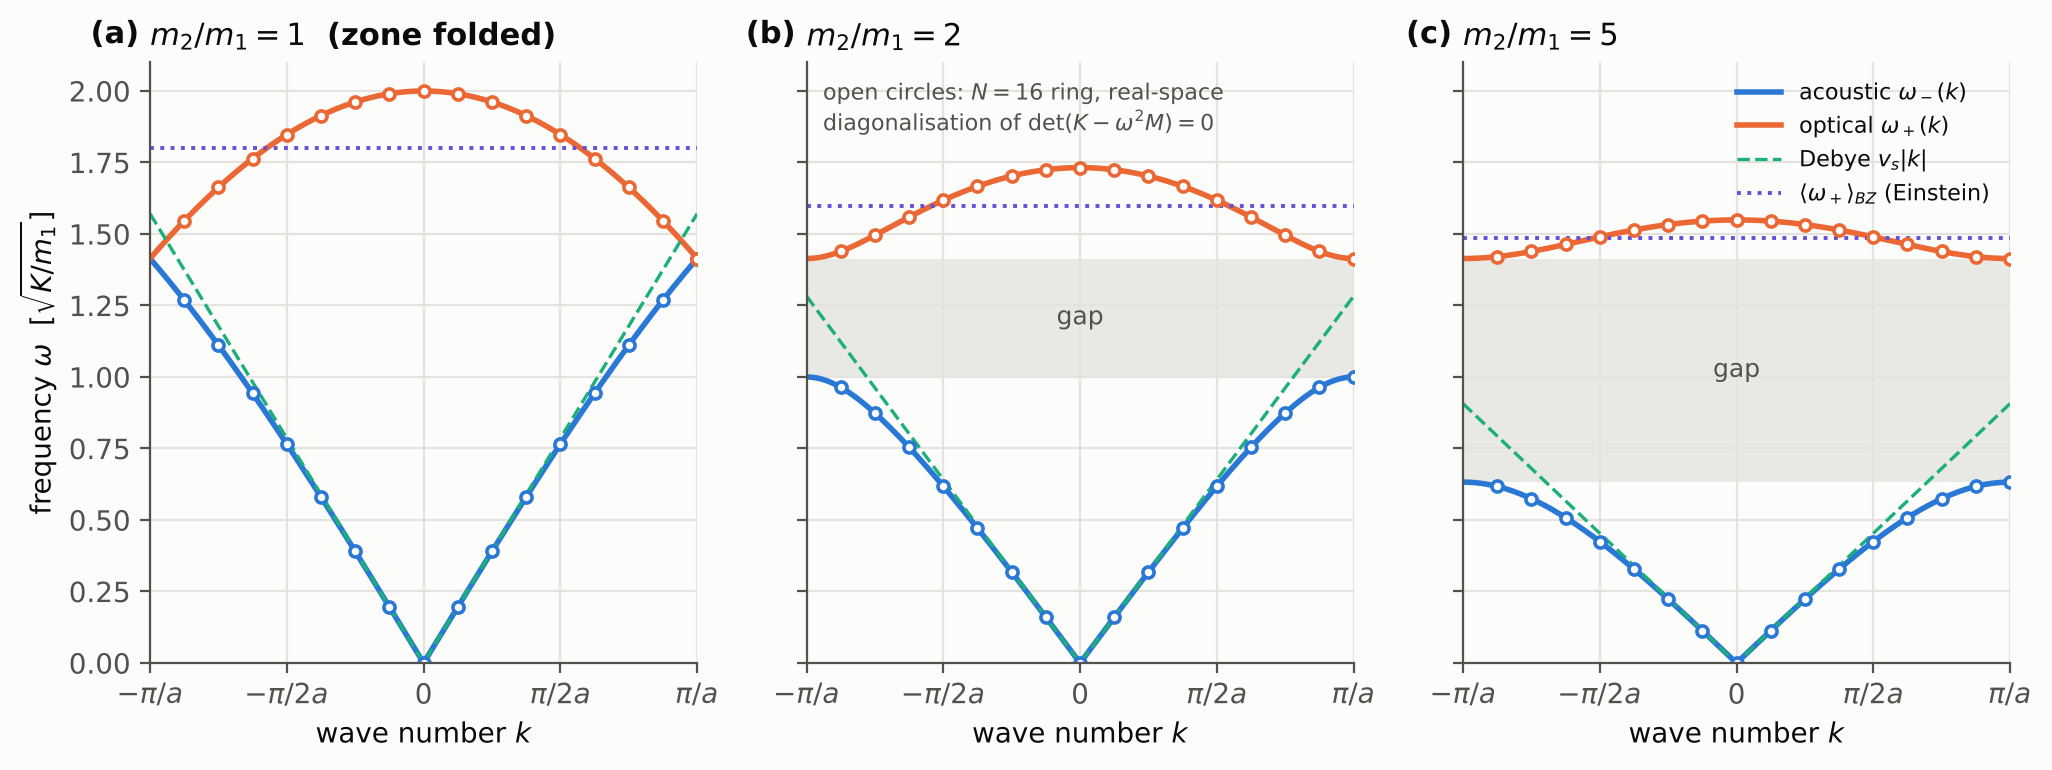
\includegraphics[width=\textwidth]{dispersion.png}
\caption{Acoustic (blue) and optical (orange) branches for three mass ratios
with $K_1=K_2$. Circles are the $2N$ frequencies of an $N=16$ ring obtained by
diagonalising $\det(K-\omega^2M)=0$ directly in real space, without Bloch's
theorem: they fall on the curves at the $N$ values of $k$ allowed by Born–von
Kármán (maximum difference $\sim2\times10^{-8}$, round-off of the translation
mode). Green: the Debye line $\vs|k|$; violet: the Einstein level
$\avg{\omega_+}_{\rm BZ}$. (a) With equal masses the gap closes: this is the
monatomic chain of spacing $a/2$ with its zone ``folded''.}
\label{fig:dispersion}
\end{figure}

\subsection{Eigenvectors: what moves in each branch}

From the first row of $(D-\omega^2)\bm e=0$, the ratio of physical amplitudes is
\begin{equation}
\frac{u_2}{u_1}=\frac{\sigma-m_1\omega^2}{K_1+K_2\ee^{-\ii ka}} .
\end{equation}
\begin{itemize}
\item At $k=0$, acoustic branch: $u_2/u_1=1$; the cell translates rigidly.
\item At $k=0$, optical branch: $u_2/u_1=-m_1/m_2$; the atoms oscillate in
  antiphase and \textbf{the centre of mass of each cell stays at rest}.
\item At $k=\pi/a$ (with $K_1=K_2$, $m_2>m_1$): in the acoustic branch only the
  heavy atoms move and in the optical branch only the light ones; each
  sublattice vibrates as if the other were a rigid wall, hence the frequencies
  $\sqrt{2K/m}$.
\end{itemize}
Fig.~\ref{fig:eigen} shows the ratio (measured from each atom's own position,
which for $K_1=K_2$ makes it real: $\frac{2K-m_1\omega^2}{2K\cos(ka/2)}$) and
the real-space patterns.

\begin{figure}[t]
\centering
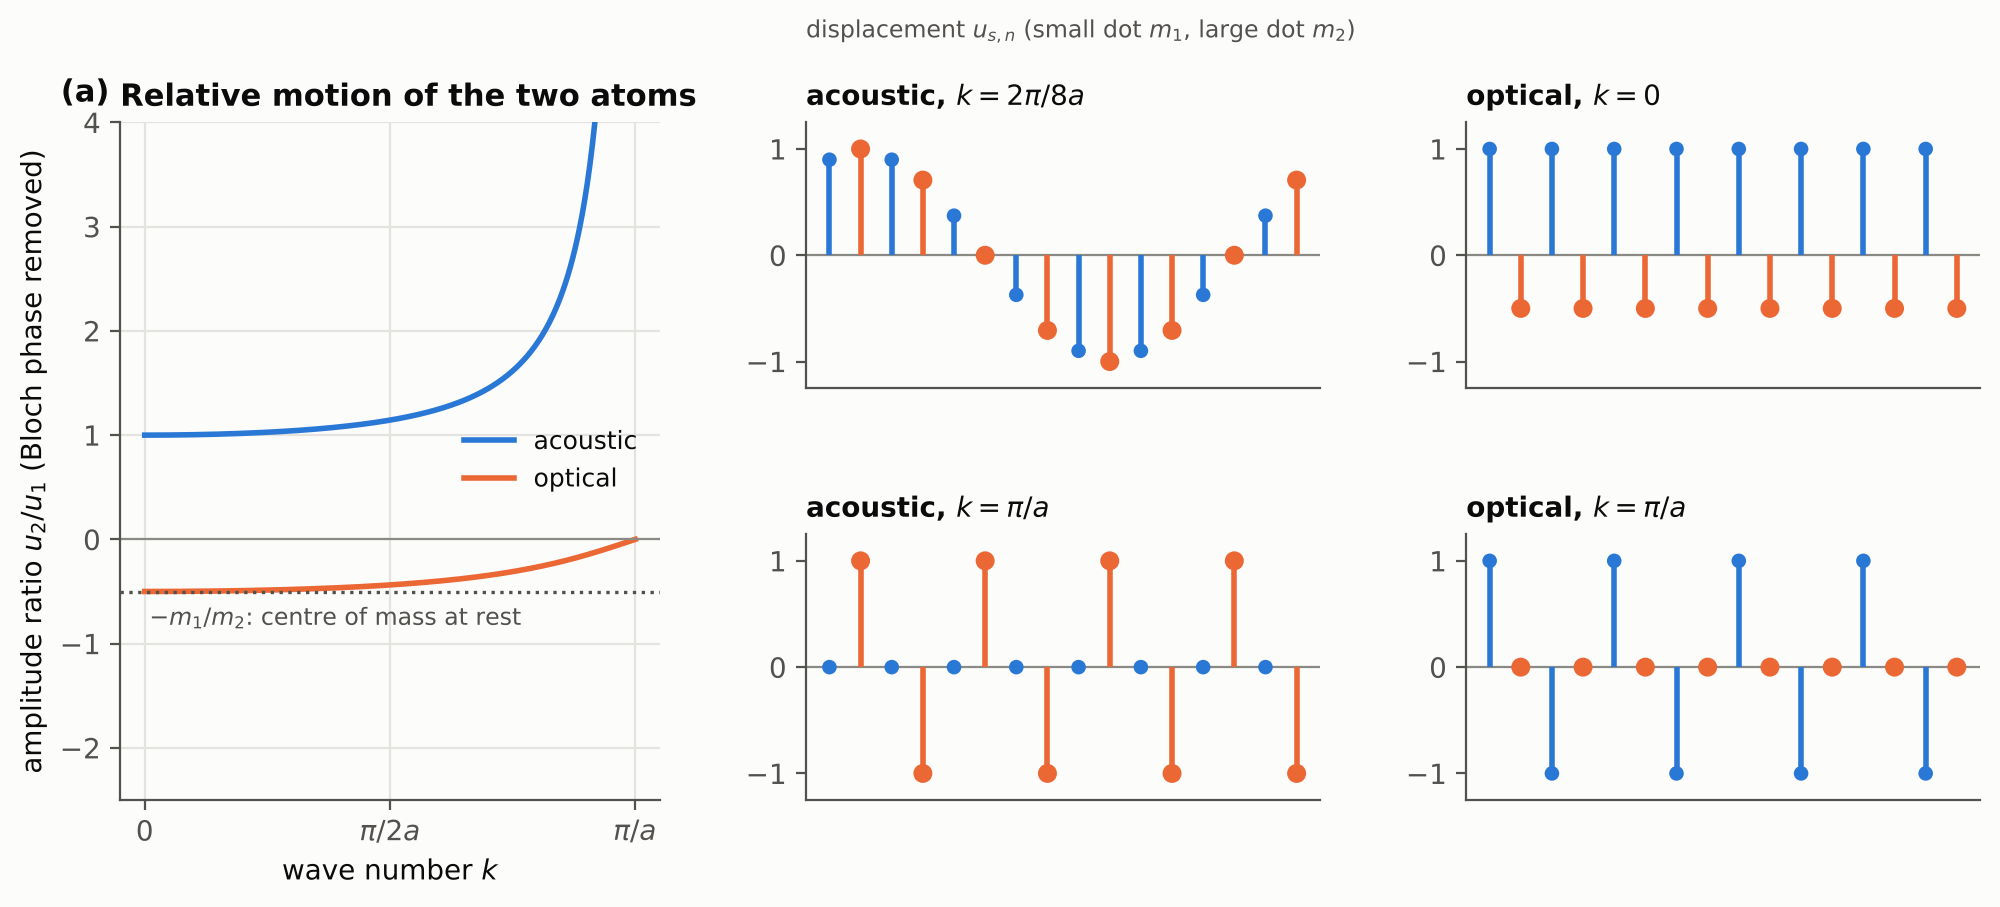
\includegraphics[width=\textwidth]{eigenvectors.png}
\caption{(a) Amplitude ratio $u_2/u_1$ across the Brillouin zone
($m_2/m_1=2$): positive (in phase) in the acoustic branch, negative (antiphase)
in the optical branch, with the value $-m_1/m_2$ at $k=0$. (b)–(e)
Displacements of the $16$ atoms of an $8$-cell ring for four representative
modes.}
\label{fig:eigen}
\end{figure}

\subsection{Limiting cases and generalisation}

\paragraph{Equal masses, $m_1=m_2$, $K_1=K_2$.} The gap closes and the two
branches are the dispersion of the monatomic chain of spacing $a'=a/2$,
$\omega=2\sqrt{K/m}\,|\sin(qa'/2)|$, ``folded'' onto the smaller Brillouin zone
of the doubled cell. Choosing a doubled cell is a decision of the \Eobs, not of
the \Eesc: the physics does not change.

\paragraph{Large mass contrast, $m_2\gg m_1$.} The optical branch becomes almost
flat, $\omega_+\simeq\sqrt{2K/m_1}$: the light atoms vibrate almost
independently in the ``cage'' of the heavy ones. This is exactly Einstein's
hypothesis, which becomes almost exact for that branch. The acoustic branch
tends to that of a monatomic chain of heavy atoms.

\paragraph{Stiffness contrast, $K_1\neq K_2$.} Even with equal masses a gap
opens (Fig.~\ref{fig:gapmap}b): it is enough that the true unit cell contains two
non-equivalent atoms. This is the phonon version of a dimerised chain.

\begin{figure}[t]
\centering
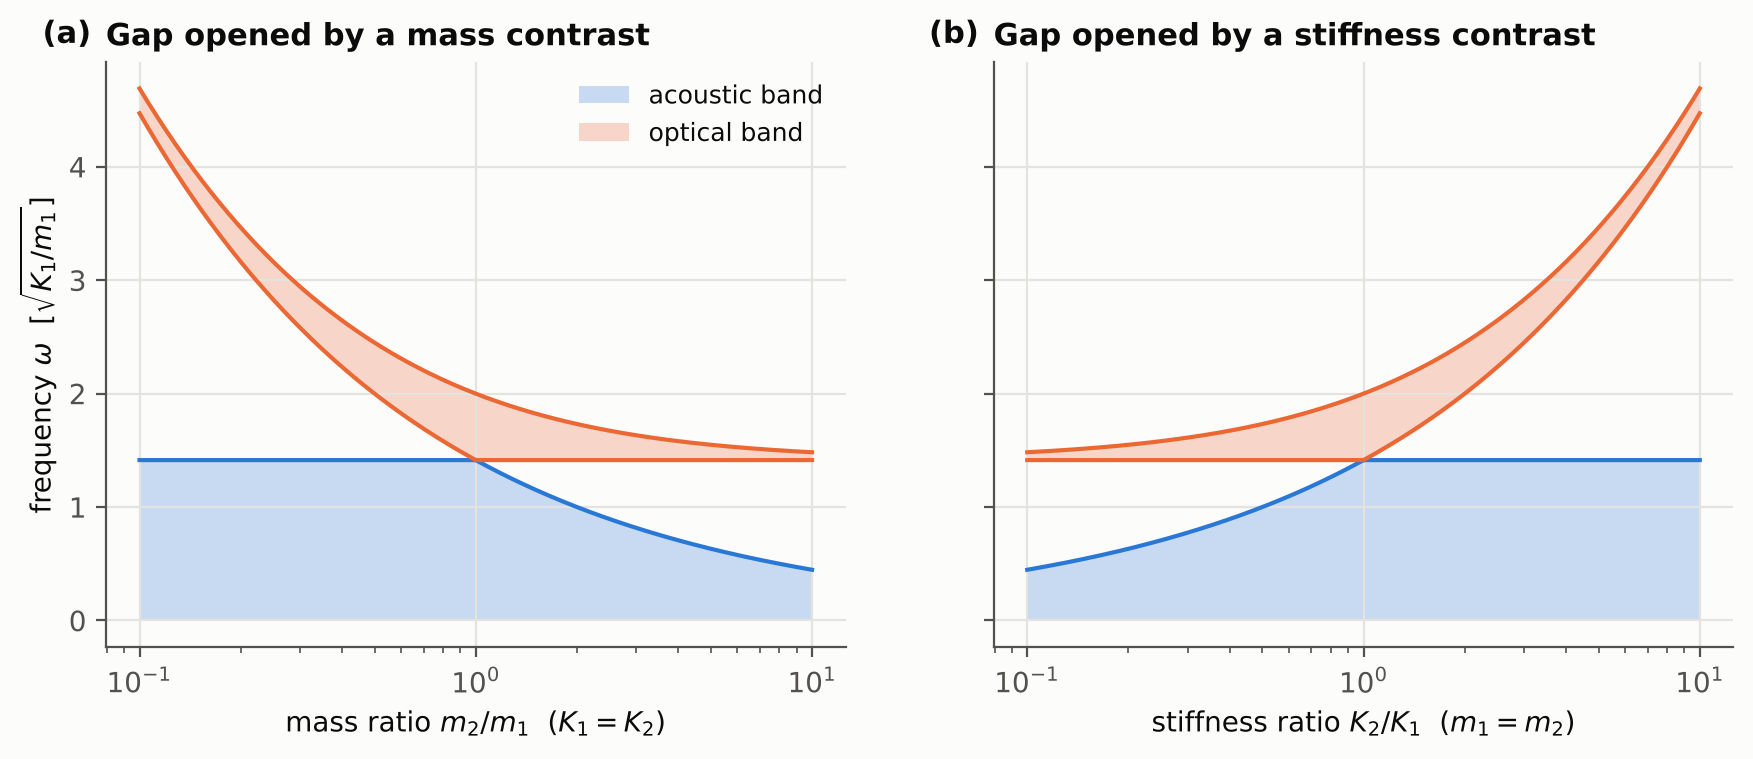
\includegraphics[width=0.92\textwidth]{gap_map.png}
\caption{Allowed bands as a function of (a) the mass ratio with $K_1=K_2$ and
(b) the stiffness ratio with $m_1=m_2$. In both cases the gap closes only when
the two atoms of the cell are equivalent.}
\label{fig:gapmap}
\end{figure}

% =====================================================================
\section{Density of states of the diatomic chain}

\subsection{Closed form}

We invert the secular equation to express $s\equiv\sin^2(ka/2)$ as a function
of $\omega$. From $\det(D-\omega^2)=0$,
$(\sigma/m_1-\omega^2)(\sigma/m_2-\omega^2)=|D_{12}|^2$, and expanding the
product the $\sigma^2$ term cancels exactly:
\begin{equation}
s(\omega)=\frac{m_1m_2\,\omega^2\left(\sigma/\mu-\omega^2\right)}{4K_1K_2}.
\end{equation}
Since $ka=2\arcsin\sqrt{s}$, $\dd k/\dd\omega=\frac{1}{a}\frac{s'(\omega)}{\sqrt{s(1-s)}}$
and, counting $\pm k$,
\begin{equation}
\boxed{\;g(\omega)=\frac{1}{\pi}\,\frac{|s'(\omega)|}{\sqrt{s(1-s)}}\,,
\qquad s'(\omega)=\frac{m_1m_2\,\omega\,(\sigma/\mu-2\omega^2)}{2K_1K_2}\,,
\qquad 0<s(\omega)<1\;}
\end{equation}
and $g=0$ outside the bands. Immediate checks:
\begin{itemize}
\item $\omega\to0$: $g(0)=\frac{a}{\pi\vs}$, the flat DOS of an elastic medium
  (the one Debye uses).
\item At the four band edges ($s=1$, or $s'=0$ at the optical top) $g$ diverges
  as $(\omega_c-\omega)^{-1/2}$: van Hove singularities.
\item The cumulative number of modes is also closed:
\begin{equation}
N(\omega)=\begin{cases}
\frac2\pi\arcsin\sqrt{s(\omega)} & \text{acoustic band}\\
1 & \text{gap}\\
2-\frac2\pi\arcsin\sqrt{s(\omega)} & \text{optical band}
\end{cases}
\end{equation}
(the optical branch \emph{decreases} with $|k|$), with $N(\infty)=2$: one
acoustic and one optical mode per cell.
\end{itemize}

\begin{codigo}
The DOS is computed along three independent routes in \code{dos.py}: the closed
form (\code{analytic\_dos}), the histogram of the frequencies on a fine $k$-grid
(\code{sampled\_dos}) and the histogram of the $2N$ eigenvalues of a finite ring
diagonalised in real space (\code{histogram\_dos}). Since $N(\omega)$ is exact,
the exact average of $g$ over each histogram bin is $\Delta N/\Delta\omega$
(\code{bin\_averaged\_dos}): the maximum difference with the sampling of
$2\times10^5$ $k$ values is $3\times10^{-4}$, and all three routes are
normalised to $2$ up to round-off.
\end{codigo}

\begin{figure}[t]
\centering
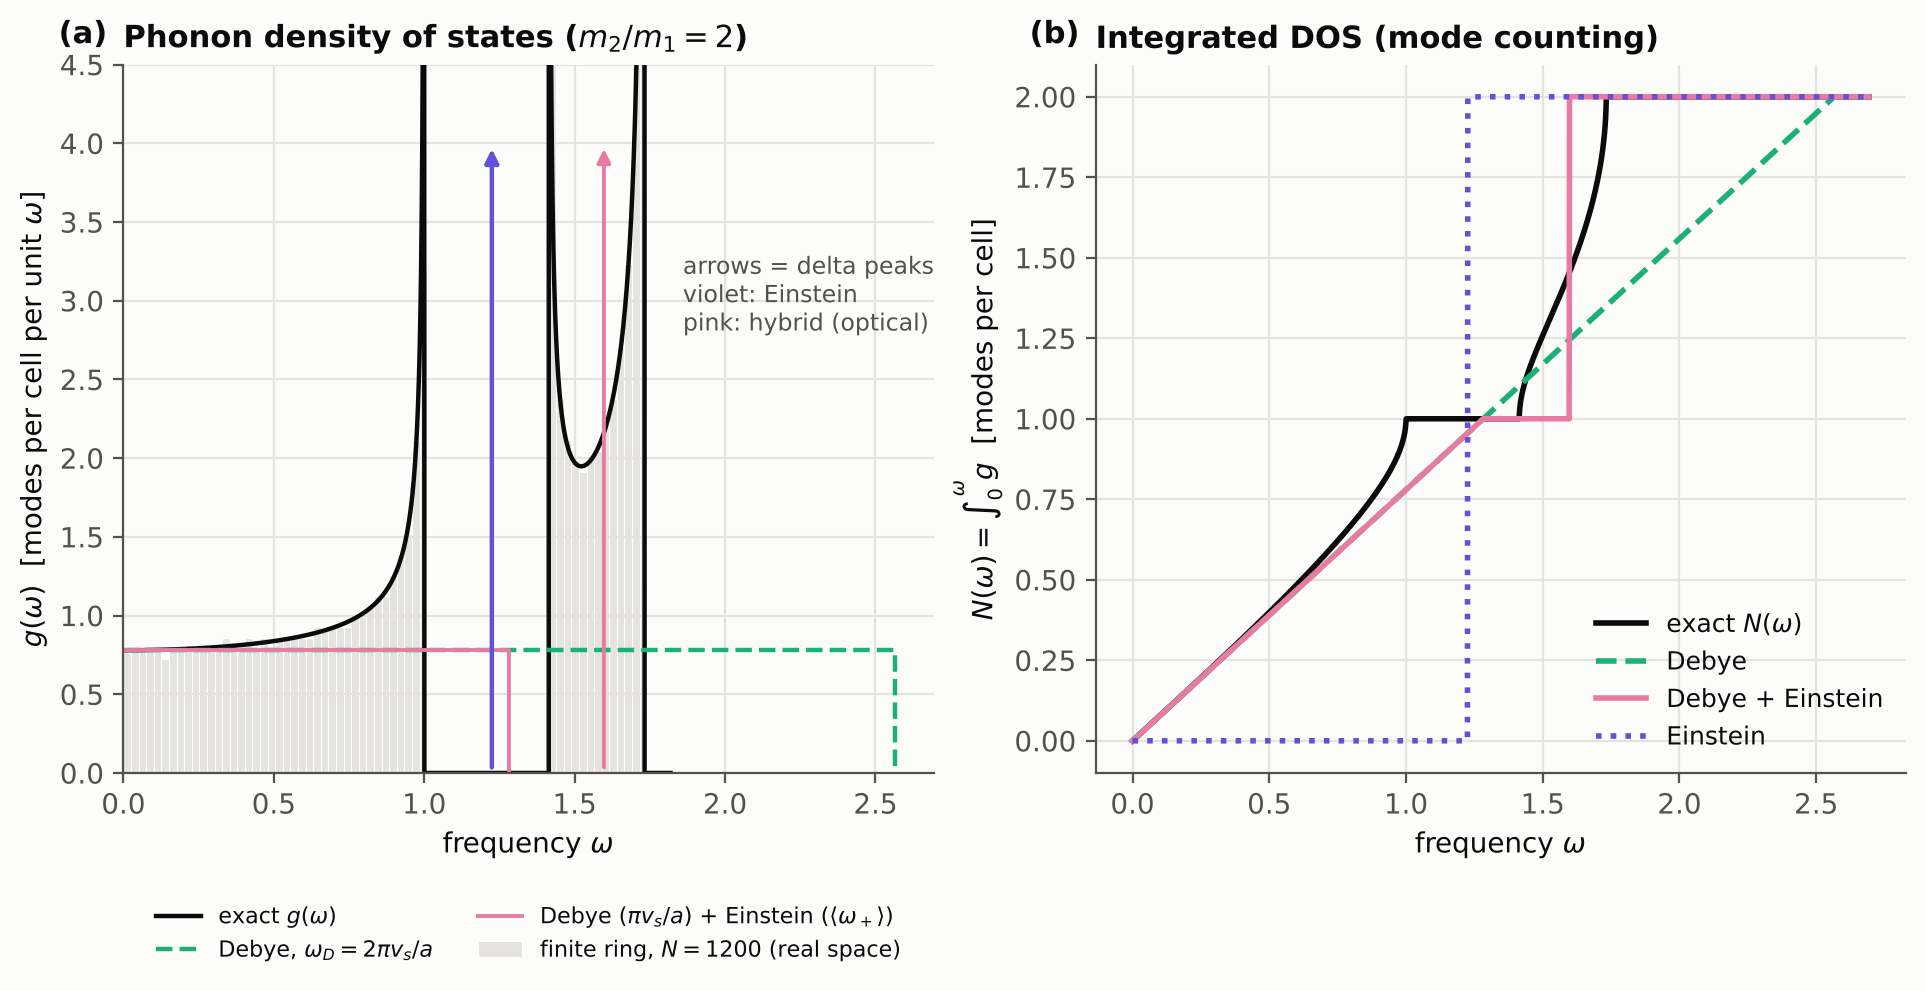
\includegraphics[width=\textwidth]{dos.png}
\caption{(a) Exact DOS (black) versus the histogram of a $1200$-cell ring
(grey), Debye's flat DOS (green), the hybrid model (pink: Debye for the
acoustic branch up to $\pi\vs/a$ plus an Einstein peak at $\avg{\omega_+}$) and
the Einstein peak (violet). (b) Cumulative number of modes: Debye spreads the
two modes per cell uniformly up to $2\pi\vs/a=2.57$, well above the real top
$1.73$.}
\label{fig:dos}
\end{figure}

\subsection{Physical reading of Fig.~\ref{fig:dos}}

The exact DOS has three features no simple model reproduces at once: the
acoustic plateau at low frequency (which Debye does capture), the pile-up of
modes at band edges (van Hove) and the gap. Debye places modes where there are
none (between $1.73$ and $2.57$) to make up the total count; Einstein places all
modes at a single frequency. Since $C_V$ is an average of $g$ weighted by
$c(\hbar\omega/\kB T)$, a smooth function, the fine details of $g$ are washed
out: the quantitative question is \emph{by how much}.

% =====================================================================
\section{Heat capacity: numerical result versus the models}

\subsection{Numerical method}

Instead of integrating \eqref{eq:dosint} over $\omega$, where $g$ is singular,
we integrate over $k$, where everything is smooth:
\begin{equation}
\frac{C_V}{N\kB}=\frac{a}{\pi}\int_0^{\pi/a}\dd k\,\sum_{b=\pm}c\!\left(\frac{\hbar\omega_b(k)}{\kB T}\right),
\end{equation}
with Gauss–Legendre quadrature (exponential convergence). At low temperature the
acoustic integrand is only appreciable for $k\lesssim 40\kB T/\hbar\vs$, so the
interval is split there to concentrate nodes where the function lives. The
result agrees with the integral over the analytic DOS
(\code{scipy.integrate.quad}) to $10^{-12}$ and with the exact sum over the
modes of a $400$-cell ring to $10^{-4}$ (finite-size effect).

\subsection{Results}

\begin{figure}[t]
\centering
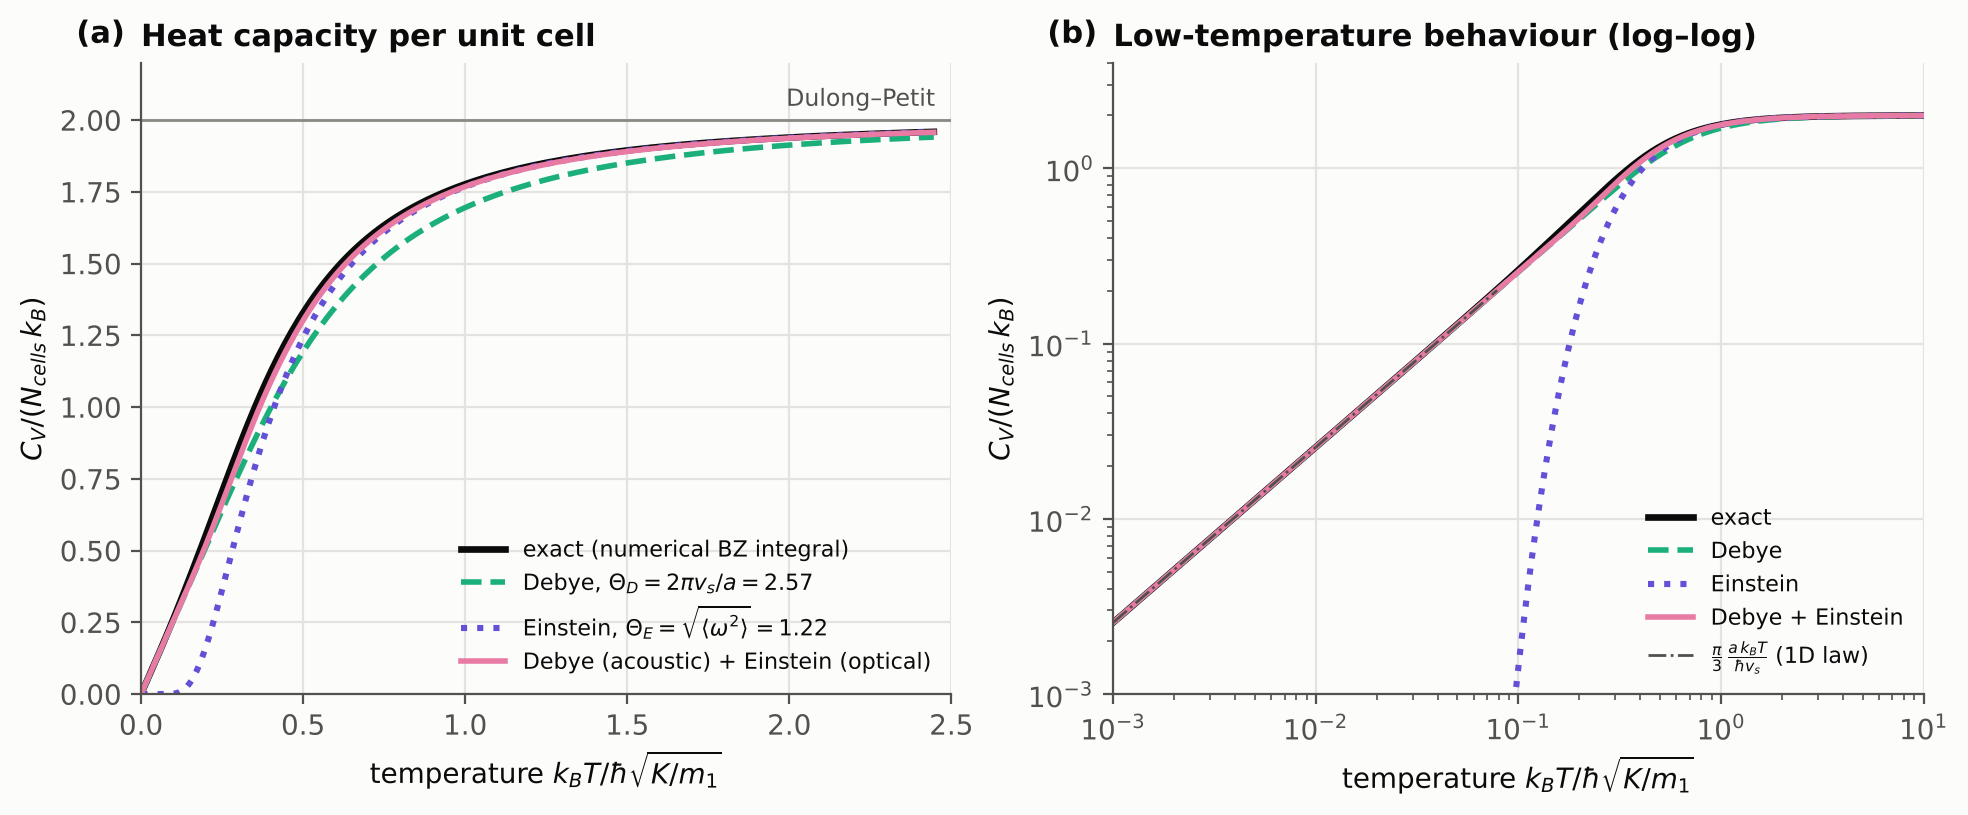
\includegraphics[width=\textwidth]{heat_capacity.png}
\caption{Heat capacity per cell of the reference chain ($m_2/m_1=2$). (a)
Linear scale: exact (black) versus Debye with $\Theta_D=2\pi\vs/a$, Einstein
with $\Theta_E=\sqrt{\avg{\omega^2}}$ and the hybrid. (b) Log–log scale: at low
$T$ the exact result follows the linear law \eqref{eq:lowT} (numerical slope
$2.56510$ versus the theoretical $\pi a/3\vs=2.56510$) while Einstein drops
exponentially.}
\label{fig:cv}
\end{figure}

\begin{table}[h]
\centering
\small
\begin{tabular}{@{}ccccc@{}}
\toprule
$\kB T$ & exact & Debye & Einstein & Debye + Einstein\\
\midrule
0.01 & 0.02566 & 0.02565 & $2\times10^{-49}$ & 0.02565\\
0.1  & 0.2629  & 0.2565  & 0.00144 & 0.2565\\
0.3  & 0.8553  & 0.7654  & 0.5816  & 0.8141\\
0.5  & 1.3286  & 1.1931  & 1.2411  & 1.3023\\
1.0  & 1.7764  & 1.6952  & 1.7677  & 1.7684\\
2.0  & 1.9393  & 1.9129  & 1.9387  & 1.9372\\
\bottomrule
\end{tabular}
\caption{$C_V/N\kB$ of the reference chain. The models use parameters fixed by
the physics (not fitted): $\Theta_D=2\pi\hbar\vs/a\kB=2.565$,
$\Theta_E=\sqrt{\avg{\omega^2}}=1.225$ and, in the hybrid,
$\omega_D^{\rm ac}=\pi\vs/a=1.283$ and $\omega_E=\avg{\omega_+}_{\rm BZ}=1.597$.}
\label{tab:cv}
\end{table}

The quantitative conclusions for $m_2/m_1=2$ are:
\begin{enumerate}
\item \textbf{Low temperature.} Debye (and hence the hybrid) is exact; the
  relative error is $2\times10^{-4}$ at $\kB T=10^{-2}$ and $2\times10^{-6}$ at
  $\kB T=10^{-3}$. Einstein fails completely (49 orders of magnitude at
  $\kB T=0.01$).
\item \textbf{High temperature.} All three tend to Dulong–Petit. Einstein with
  $\omega_E^2=\avg{\omega^2}$ reproduces by construction the $1/T^2$
  correction (at $\kB T=10$: exact $1.997503$, expansion $1.997500$) and is the
  best of the three above $\kB T\approx1$.
\item \textbf{Intermediate region} ($\kB T\sim0.1$–$0.5$, where $C_V$ rises
  fastest). Here lives the physics of the real DOS: Debye underestimates $C_V$
  by up to $11\%$ because it spreads modes up to $2.57$, where they are still
  frozen; the hybrid reduces the maximum error to $6\%$.
\item \textbf{Fits.} Least-squares fitting a single $\Theta$ over
  $\kB T\in[0.02,3]$: Debye gives $\Theta_D=2.256$ with rms error $0.020$, but
  then it is no longer exact at low $T$ (maximum relative error $14\%$);
  Einstein gives $\Theta_E=0.962$ with rms error $0.14$ and still fails
  qualitatively at low $T$. A good global fit does not imply good physics: the
  fitted parameter hides the structure of $g(\omega)$.
\end{enumerate}

\subsection{Branch decomposition}

\begin{figure}[t]
\centering
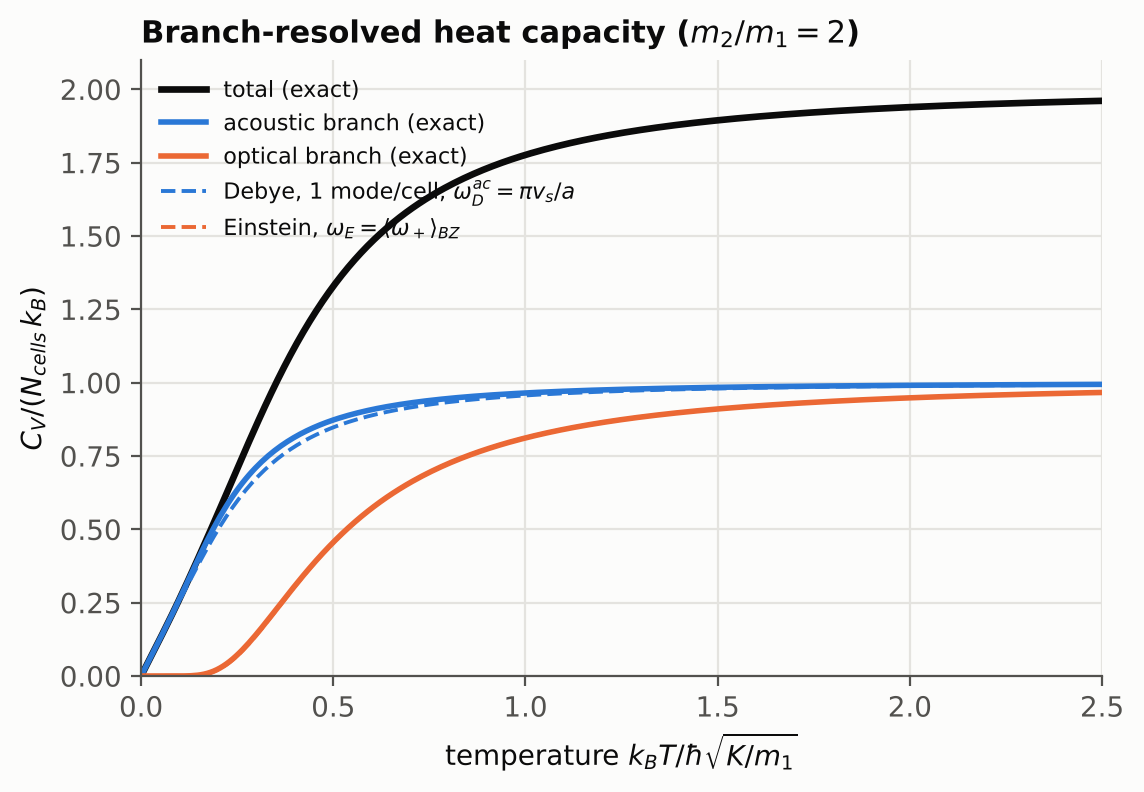
\includegraphics[width=0.62\textwidth]{heat_capacity_branches.png}
\caption{Acoustic and optical contributions to the heat capacity (each saturates
at $\kB$ per cell) and the Debye (1 mode/cell) and Einstein models applied to
each branch separately.}
\label{fig:branches}
\end{figure}

Since the system is ideal, $C_V=C_{\rm ac}+C_{\rm op}$ exactly
(Fig.~\ref{fig:branches}). The optical branch is frozen below
$\kB T\approx0.1$ (it contributes $0.02\%$ of $C_V$ at $\kB T=0.1$), $10\%$ at
$\kB T=0.25$ and $34\%$ at $\kB T=0.5$. All low-temperature physics is
acoustic, which justifies the hybrid model: Debye where the dispersion is
linear, Einstein where the branch is narrow. The figure also shows where the
hybrid's error lives: in the acoustic part, because the real branch bends (and
piles up modes at its top) while Debye keeps it linear.

\subsection{Dependence on the mass ratio}

\begin{figure}[t]
\centering
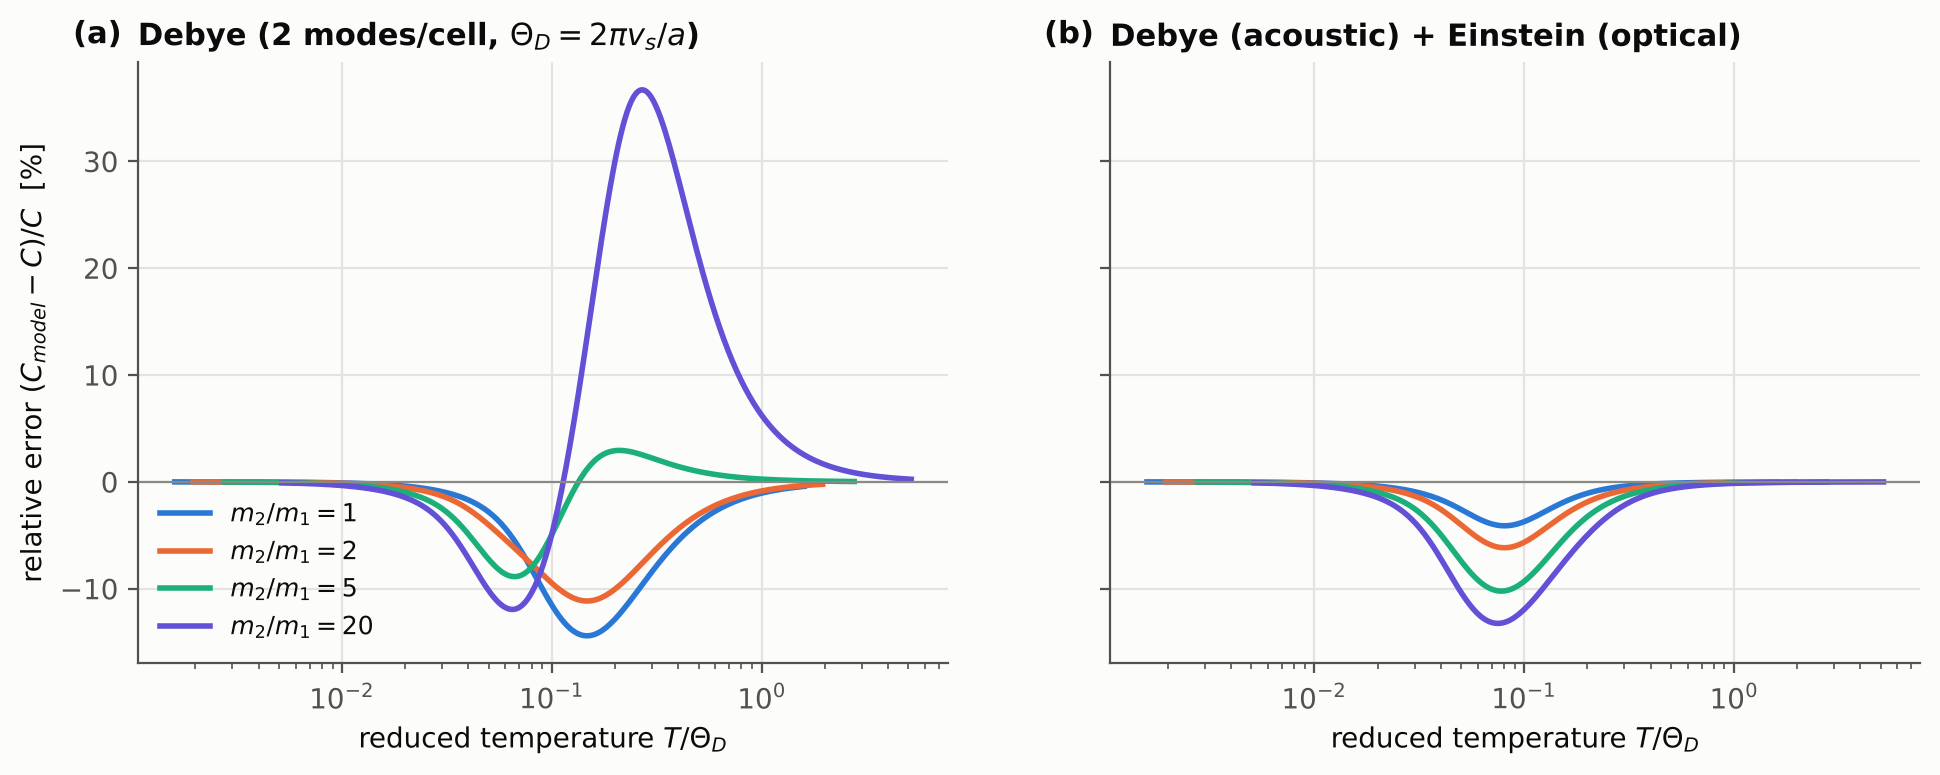
\includegraphics[width=\textwidth]{model_errors.png}
\caption{Relative error of (a) Debye and (b) the hybrid model versus $T/\Theta_D$
for several mass ratios.}
\label{fig:errors}
\end{figure}

Fig.~\ref{fig:errors} summarises how the quality of the models changes with
$m_2/m_1$:
\begin{center}
\small
\begin{tabular}{@{}ccc@{}}
\toprule
$m_2/m_1$ & max.\ error Debye & max.\ error Debye + Einstein\\
\midrule
1  & $14.4\%$ & $4.1\%$\\
2  & $11.2\%$ & $6.2\%$\\
5  & $8.9\%$  & $10.2\%$\\
20 & $36.7\%$ & $13.2\%$\\
\bottomrule
\end{tabular}
\end{center}
\begin{itemize}
\item \textbf{Debye} degrades dramatically for large contrasts: the heavier the
  second atom, the smaller $\vs$, the smaller $\Theta_D$ and the worse it
  describes the optical branch, whose frequency $\sqrt{2K/m_1}$ does not depend
  on $m_2$. For $m_2/m_1=20$ it overestimates $C_V$ by $37\%$ (it lets optical
  modes vibrate that are actually frozen).
\item \textbf{The hybrid} shows an apparently paradoxical trend: its error
  \emph{grows} with $m_2/m_1$ even though the optical branch gets flatter and
  flatter (Einstein becomes more and more exact). The reason is that the
  residual error is Debye's error on the acoustic branch, which for large
  contrast is that of a monatomic chain of heavy atoms, sinusoidal and with a
  strong van Hove singularity at its top; its Debye error is $\simeq14\%$, the
  same as for the monatomic chain in the first row. For $m_2/m_1=1$ the hybrid
  is very good because the ``optical branch'' is the folded upper half of the
  same sinusoid and $\avg{\omega_+}$ represents it well.
\end{itemize}

\subsection{Effective Debye temperature}

\begin{figure}[t]
\centering
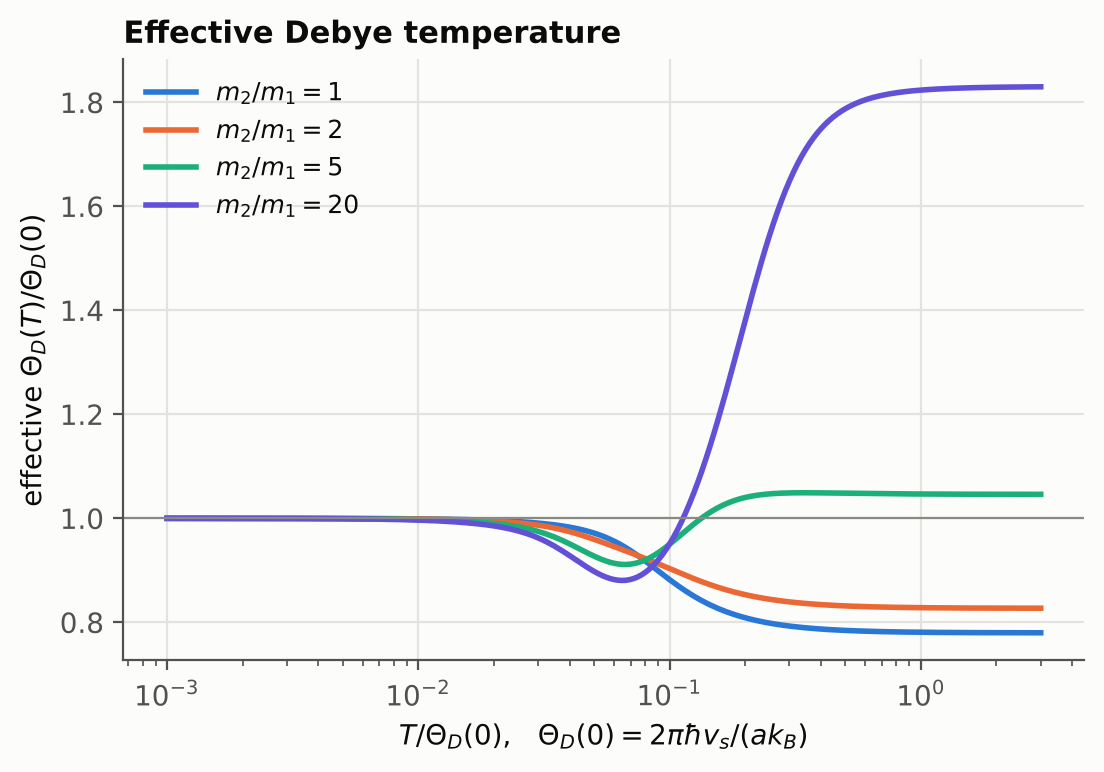
\includegraphics[width=0.62\textwidth]{debye_temperature.png}
\caption{Effective Debye temperature $\Theta_D(T)$, normalised to its $T=0$
value, for several mass ratios.}
\label{fig:thetaD}
\end{figure}

Fig.~\ref{fig:thetaD} shows $\Theta_D(T)/\Theta_D(0)$. All curves start at $1$
(Debye exact as $T\to0$) and drop as soon as the acoustic modes near the top of
the band are excited: the real DOS piles them up below the Debye cutoff (van
Hove) and the crystal ``softens''. For $m_2/m_1=1$ and $2$ the drop is
monotonic; for $m_2/m_1=5$ and $20$ there is a minimum near
$T\approx0.06\,\Theta_D(0)$ followed by a rise, when the optical branch
unfreezes. At high temperature all of them saturate at
$\sqrt{3\avg{\omega^2}}/\Theta_D(0)$: $0.78$, $0.83$, $1.05$ and $1.83$ for
$m_2/m_1=1,2,5,20$. For large contrasts the saturation exceeds $1$: the optical
branch, high in frequency and holding half of the modes, ``stiffens'' the
crystal compared with what the sound velocity predicts. This is exactly what is
observed experimentally in solids with very different masses in the basis, and
the reason why a single tabulated Debye temperature never describes the whole
temperature range well.

% =====================================================================
\section{Other observables}

\subsection{Internal energy, entropy and free energy}

\begin{figure}[t]
\centering
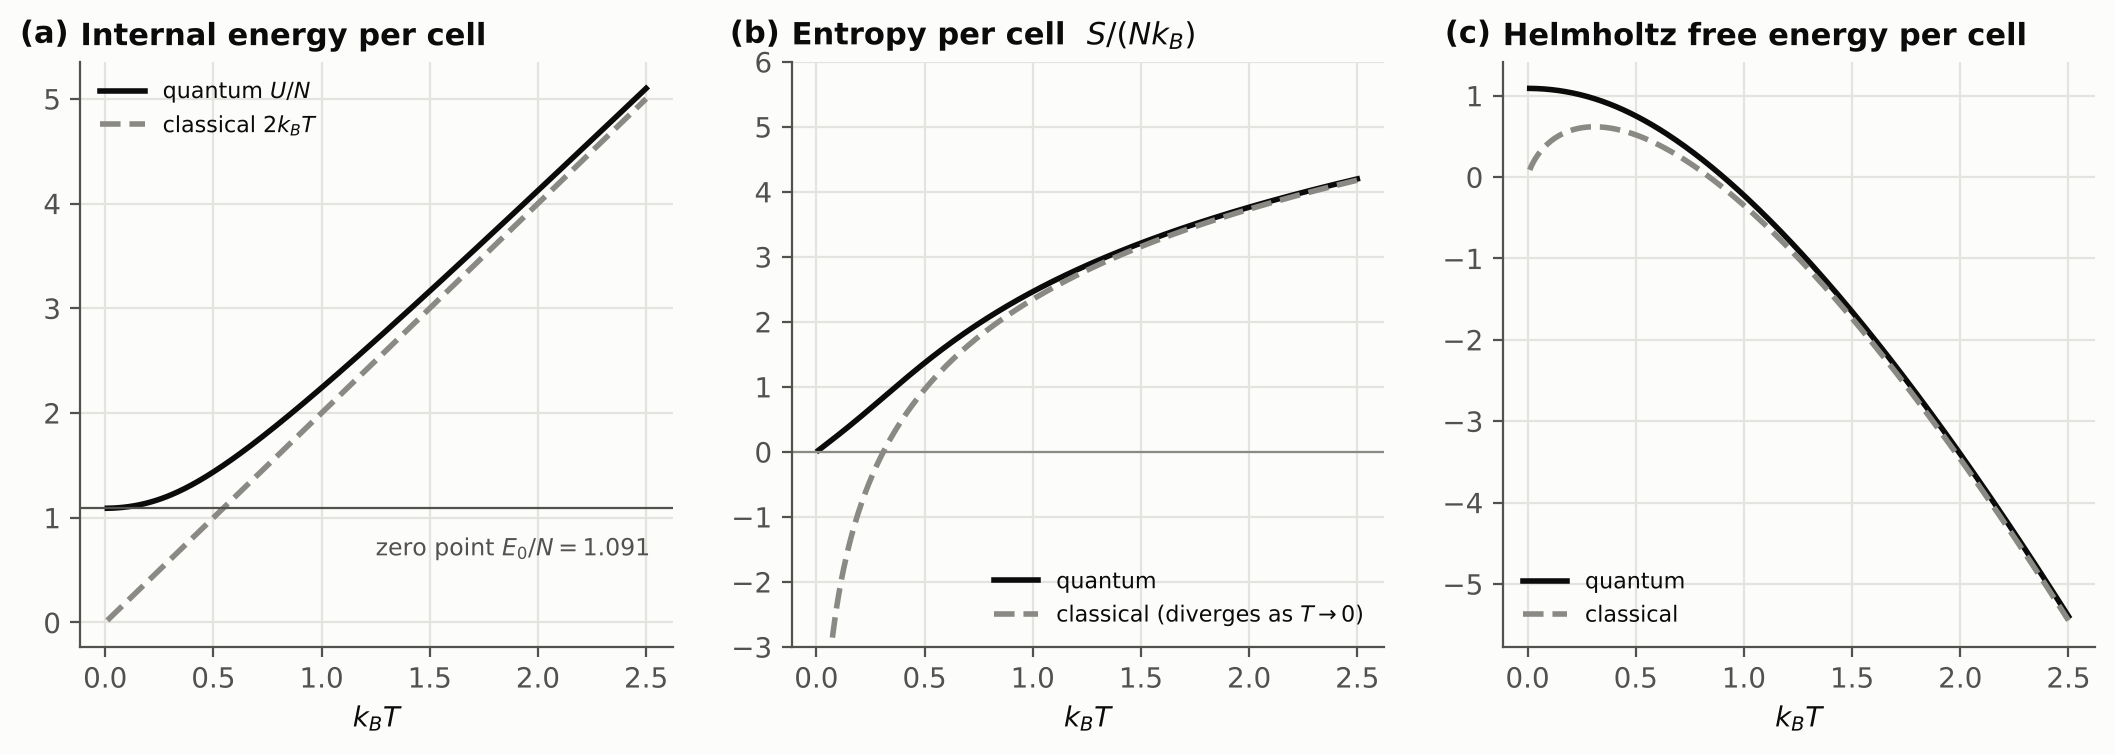
\includegraphics[width=\textwidth]{thermo_functions.png}
\caption{(a) Internal energy per cell: at $T=0$ the zero-point energy
$E_0/N=1.091$ remains; at high $T$ the quantum curve tends to the classical
$2\kB T$ (not to $2\kB T+E_0/N$: the zero point cancels in the expansion
$\frac{\hbar\omega}{2}\coth\frac{y}{2}=\kB T+\frac{\hbar^2\omega^2}{12\kB T}+\dots$).
(b) Entropy: the quantum one vanishes at $T=0$ (third law); the classical one
diverges to $-\infty$, a sign that classical counting of microstates fails at
low temperature. (c) Helmholtz free energy.}
\label{fig:thermo}
\end{figure}

Fig.~\ref{fig:thermo} shows $U$, $S$ and $F$ per cell in the quantum and
classical treatments. Two statistical-mechanics remarks: (i) the negative
classical entropy at low $T$ is the same symptom as the negative Sackur–Tetrode
entropy at low temperature: discretising phase space into cells of volume $h$
stops making sense when the typical action is of order $\hbar$; (ii)
thermodynamic consistency $S=-\partial F/\partial T$, $C_V=\partial U/\partial T$,
$U=F+TS$ is checked numerically in the tests to $10^{-6}$.

\subsection{Displacement fluctuations: no long-range order in 1D}

This is the most interesting observable physically. Expanding in normal modes,
$u_{s,n}=N^{-1/2}\sum_{k,b}(e_s/\sqrt{m_s})\ee^{\ii kna}Q_{k,b}$, and using that
each normal coordinate is a unit-mass oscillator with
\begin{equation}
\avg{|Q_{k,b}|^2}=\frac{\hbar}{2\omega}\coth\frac{\hbar\omega}{2\kB T}
\ \xrightarrow{\ \hbar\to0\ }\ \frac{\kB T}{\omega^2},
\end{equation}
we compute the \textbf{mean-square relative displacement} of two atoms $r$
cells apart,
\begin{equation}
G_{ss'}(r)=\avg{(u_{s',n+r}-u_{s,n})^2}
=\frac{a}{2\pi}\int_{\rm BZ}\dd k\sum_b\avg{|Q_{k,b}|^2}
\left|\frac{e_{s'}\ee^{\ii kra}}{\sqrt{m_{s'}}}-\frac{e_s}{\sqrt{m_s}}\right|^2 .
\end{equation}
The factor $|\cdots|^2\propto k^2$ of the acoustic branch as $k\to0$ makes
$G(r)$ finite for each $r$, but its dependence on $r$ is very revealing
(Fig.~\ref{fig:disp}a):
\begin{itemize}
\item \textbf{Classically} the result is exact and simple:
  $G_{11}(r)=r\,\kB T\left(\frac{1}{K_1}+\frac{1}{K_2}\right)$. The bond stretches
  are independent Gaussian variables of variance $\kB T/K_i$ (equipartition
  applied to each spring), and the separation between two atoms is the sum of
  $2r$ of them: a random walk. The code reproduces it with relative error
  $<10^{-8}$.
\item \textbf{Quantum, at $T=0$}, $G(r)\simeq\frac{\hbar a}{\pi M\vs}\ln r$:
  logarithmic growth (numerical slope $0.259899$ versus the theoretical
  $0.259899$).
\end{itemize}
Since $G(r)\to\infty$ as $r\to\infty$, the positions of distant atoms are
uncorrelated: \textbf{a 1D chain has no long-range positional order} at any
temperature (Landau–Peierls argument). It is the same moral as the absence of a
phase transition in the 1D Ising model: in one dimension long-wavelength
fluctuations always win. Equivalently, the mean-square displacement of one atom
in a ring of $N$ cells (with the rigid translation removed) diverges with $N$
(Fig.~\ref{fig:disp}b): $\avg{u_1^2}=\frac{N}{12}\kB T\left(\frac1{K_1}+\frac1{K_2}\right)$
classically (checked: $0.166667\,N\kB T$ for our parameters) and
$\simeq\frac{\hbar a}{2\pi M\vs}\ln N$ at $T=0$. The Debye–Waller factor
$\ee^{-q^2\avg{u^2}}$ vanishes in the thermodynamic limit: a 1D crystal would
not give sharp Bragg peaks.

\begin{figure}[t]
\centering
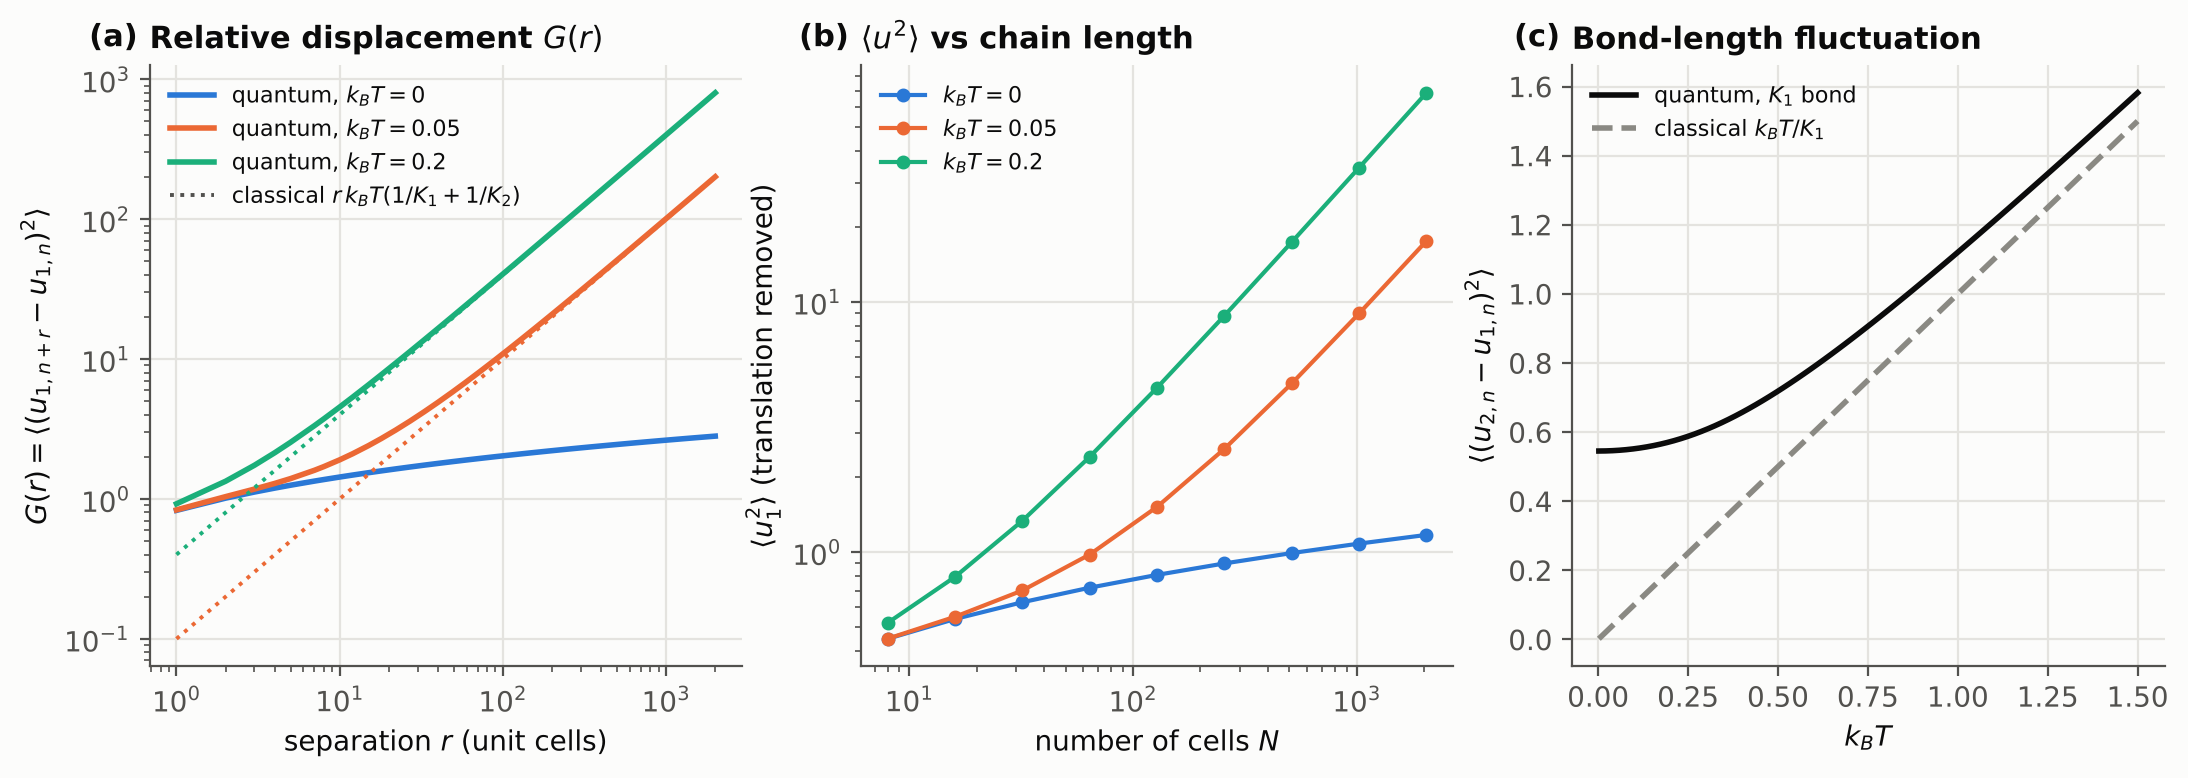
\includegraphics[width=\textwidth]{displacements.png}
\caption{(a) Quantum relative displacement $G(r)$ at three temperatures (solid)
and the classical result $r\kB T(1/K_1+1/K_2)$ (dotted): at short distances the
zero point dominates, at long distances the thermal linear growth. (b)
$\avg{u_1^2}$ in rings of $N$ cells: linear in $N$ at $T>0$, logarithmic at
$T=0$. (c) Bond fluctuation: the zero point ($0.545$ at $T=0$) versus the
classical line $\kB T/K_1$.}
\label{fig:disp}
\end{figure}

\subsection{Bond fluctuation}

\emph{Local} fluctuations, on the other hand, are well defined: the fluctuation
of the $K_1$ bond, $\avg{(u_{2,n}-u_{1,n})^2}$, is finite at every temperature
(Fig.~\ref{fig:disp}c). At $T=0$ it equals $0.545$ (in units of
$\hbar/\sqrt{Km_1}$) because of zero-point motion, and at high $T$ it tends to
equipartition, $\kB T/K_1$. This is the quantity entering a Lindemann-type
melting criterion, and it again shows the crossover from the quantum regime
(plateau) to the classical one (straight line).

% =====================================================================
\section{Independent validation: Langevin dynamics}\label{sec:langevin}

\subsection{Motivation}

Everything above uses normal modes. To test the physics along a completely
different route we simulate the \emph{classical} dynamics of a ring of atoms
coupled to a heat bath through the Langevin equation:
\begin{equation}
\dd q_i=\frac{p_i}{m_i}\dd t,\qquad
\dd p_i=F_i(q)\,\dd t-\gamma p_i\,\dd t+\sqrt{2m_i\gamma\kB T}\;\dd W_i ,
\end{equation}
with $\dd W_i$ Wiener increments (white noise). The dissipative force
$-\gamma p$ and the stochastic one balance on average (Einstein relation between
friction and diffusion) and the stationary distribution is the canonical one.

As stressed in \S\ref{sec:normales}, an isolated harmonic chain is integrable:
a single microcanonical (NVE) trajectory would never sample the canonical
ensemble because each mode keeps its energy. The Langevin bath supplies the
``residual interaction'' that thermalises each mode.

\subsection{Integrator}

We use the BAOAB splitting (Leimkuhler and Matthews, 2013):
\[
\text{B: } p\mathrel{+}=\tfrac{\Delta t}{2}F,\quad
\text{A: } q\mathrel{+}=\tfrac{\Delta t}{2}\tfrac{p}{m},\quad
\text{O: } p\leftarrow c\,p+\sqrt{(1-c^2)m\kB T}\,\xi,\quad
\text{A},\quad \text{B},
\qquad c=\ee^{-\gamma\Delta t},
\]
with independent normal $\xi$. For $\gamma=0$ it reduces exactly to the
\textbf{velocity Verlet} algorithm, which is symplectic (it preserves phase-space
volume, consistently with Liouville's equation); the test
\code{test\_velocity\_verlet\_conserves\_energy} checks energy conservation to
$10^{-3}$ after $5000$ steps. With $\gamma>0$, BAOAB samples configurational
averages with a very small time-step error.

\subsection{Three measurements and their exact predictions}

\paragraph{DOS from the velocity spectrum.} By the Wiener–Khinchin theorem, the
spectral density of each atom's velocity is the Fourier transform of its
autocorrelation. In equilibrium every mode has mean kinetic energy $\kB T/2$
(equipartition), so the mass-weighted spectrum
$\sum_i m_i|\tilde v_i(\omega)|^2$ is proportional to $g(\omega)$, broadened by
friction (each line is approximately a Lorentzian of half-width $\gamma/2$).
With $N=256$ cells (mode spacing $\approx0.01<\gamma=0.03$) the spectrum
reproduces the broadened exact DOS, including the van Hove singularities and the
gap (Fig.~\ref{fig:langevin}a).

\paragraph{Heat capacity from fluctuations.} Through the fluctuation–response
relation, $C_V=(\Delta E)^2/\kB T^2$. For a classical ring of $N$ cells,
counting quadratic terms ($2N$ kinetic and $2N-1$ independent potential ones,
because the stretches sum to zero around the ring), the exact value is
$C_V/N\kB=2-1/2N=1.9922$ for $N=64$. The simulation gives $1.956\pm0.023$
(block-averaging error).

\paragraph{Relative displacement on the ring.} On a ring the stretches are
independent Gaussians conditioned to sum to zero: a discrete ``Brownian
bridge'', with
\begin{equation}
G(r)=r\left(1-\frac rN\right)\kB T\left(\frac1{K_1}+\frac1{K_2}\right),
\end{equation}
which the simulation reproduces with a maximum relative deviation of $3\%$
(Fig.~\ref{fig:langevin}b). The kinetic temperatures of the two sublattices are
$0.998$ and $0.996$ (equipartition, independent of mass) and the bond variances
$0.991$ and $0.989$ versus the exact $0.992$.

\begin{figure}[t]
\centering
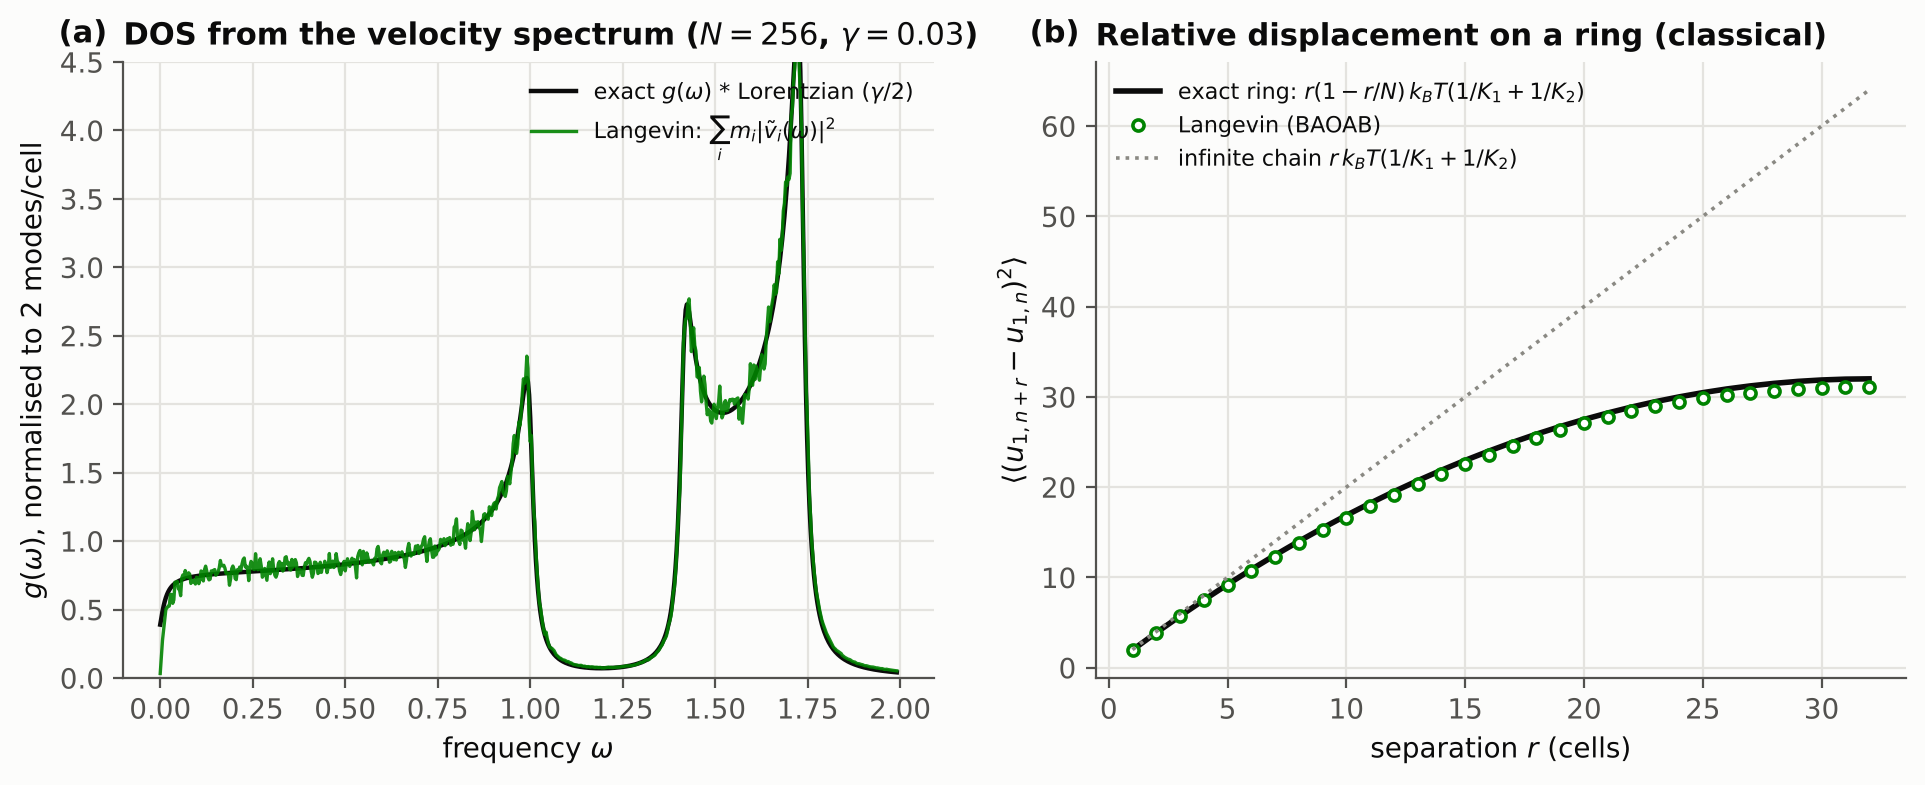
\includegraphics[width=\textwidth]{langevin.png}
\caption{Langevin dynamics (BAOAB, $\Delta t=0.05$, $\kB T=1$). (a)
Mass-weighted velocity spectrum ($N=256$, $\gamma=0.03$) versus the exact DOS
convolved with a Lorentzian of half-width $\gamma/2$. (b) Relative displacement
on a 64-cell ring ($\gamma=0.5$) versus the exact Brownian-bridge prediction and
the infinite-chain straight line.}
\label{fig:langevin}
\end{figure}

% =====================================================================
\section{Numerical implementation}

\subsection{Code structure}

\begin{center}
\small
\begin{tabularx}{\textwidth}{@{}l X@{}}
\toprule
Module & Content\\
\midrule
\code{parameters.py} & \code{ChainParameters}: immutable \code{dataclass} with $m_1,m_2,K_1,K_2,a$ and derived quantities ($\vs$, gap, $\avg{\omega^2}$, \dots).\\
\code{dispersion.py} & $D(k)$, closed-form branches (Vieta form), eigenvectors, amplitude ratio, group velocity, Born–von Kármán grid.\\
\code{real\_space.py} & $M$ and $K$ matrices of a ring or open chain and solution of $\det(K-\omega^2M)=0$ (\code{scipy.linalg.eigh}).\\
\code{dos.py} & Closed-form DOS, closed-form $N(\omega)$, histograms ($k$-grid and real space), broadened DOS, Debye DOS.\\
\code{thermodynamics.py} & Numerically stable single-oscillator functions (\code{expm1}), Gauss–Legendre quadrature in $k$, $U,C_V,F,S$, branch decomposition, asymptotics.\\
\code{models.py} & 1D Debye function, Debye, Einstein and hybrid models, characteristic frequencies, fits, $\Theta_D(T)$.\\
\code{observables.py} & $G_{ss'}(r)$ with composite quadrature, $\avg{u_s^2}$ on finite rings, bond fluctuations.\\
\code{langevin.py} & BAOAB integrator, full simulation with estimators and exact ring predictions.\\
\code{plotting.py} & Common figure style.\\
\bottomrule
\end{tabularx}
\end{center}

\subsection{Numerical subtleties}

\begin{itemize}
\item \textbf{Cancellations.} $\omega_-^2$ is computed as $\det D/\omega_+^2$ and
  $s(\omega)$ in its expanded form; both avoid subtracting nearly equal numbers
  and keep machine relative precision as $k\to0$ or $\omega\to0$. The
  eigenvectors from \code{eigh} are combined with the closed-form eigenvalues
  for the same reason.
\item \textbf{Integrating over $k$, not $\omega$.} The integrand in $k$ is
  analytic; in $\omega$ it has $(\omega_c-\omega)^{-1/2}$ singularities.
\item \textbf{Low temperature.} The Gauss–Legendre grid is split at
  $k_c=40\kB T/\hbar\vs$. The slope $C_V/T$ at $\kB T=10^{-4}$ matches the
  theoretical one to $7$ digits.
\item \textbf{Oscillating integrands.} $G(r)$ contains $\ee^{\ii kra}$; a
  composite rule is used with a number of panels growing with $r$ (linear cost in
  $r$, instead of the cubic cost of a high-order Gauss–Legendre rule).
\item \textbf{Reproducibility.} Langevin noise uses \code{numpy.random.Generator}
  with a fixed seed; every number in this document comes from
  \code{scripts/make\_figures.py}, which stores it in
  \code{results/results.json}.
\end{itemize}

\subsection{Tests}

\code{tests/test\_physics.py} contains 26 tests comparing the code with
\emph{independent} results: closed form versus diagonalisation, real space
versus Bloch, acoustic sum rule, monatomic limit, trace and second moment,
normalisation and derivative of $N(\omega)$, limits of $C_V$, DOS versus
$k$-quadrature versus finite ring, thermodynamic consistency, limits of the
Debye function, $\Theta_D(\infty)$, exact classical random walk, logarithmic
growth at $T=0$, equipartition and energy conservation in Verlet. Run them with
\code{pytest} or with \code{python tests/run\_tests.py}.

% =====================================================================
\section{Discussion and conclusions}

\begin{enumerate}
\item \textbf{From the general to the particular.} The discrete translation
  symmetry of the \Eesc{} turns a problem of $2N$ coupled degrees of freedom
  into $N$ problems of size $2\times2$; the harmonic approximation turns the
  crystal into an ideal system of oscillators, and the canonical ensemble makes
  the whole thermodynamics depend only on $g(\omega)$. The diatomic chain is the
  minimal example in which all the ingredients of a real crystal appear:
  acoustic and optical branches, gap, van Hove singularities and a DOS that is
  neither Debye's nor Einstein's.
\item \textbf{Branches.} The acoustic branch is the dynamical manifestation of
  translational invariance (sum rule); the optical branch exists because there is
  more than one atom per cell, and the gap because those atoms are not
  equivalent (different mass or stiffness).
\item \textbf{Heat capacity.} Debye is exact at low temperature (only $\vs$
  matters) and Einstein with $\omega_E^2=\avg{\omega^2}$ is exact in the first
  high-temperature correction. Neither describes the intermediate region, which
  is where the real DOS shows up: maximum errors of $11\%$ (Debye) and $6\%$
  (hybrid) for $m_2/m_1=2$.
\item \textbf{Models and mass ratio.} Debye degrades quickly with mass contrast
  ($37\%$ for $m_2/m_1=20$) because the optical scale is not set by the sound
  velocity. The hybrid greatly improves that case but keeps an irreducible
  $\sim14\%$ error, Debye's error on a sinusoidal acoustic branch. The effective
  Debye temperature varies between $0.78$ and $1.83$ times its $T=0$ value
  depending on the contrast: a single $\Theta_D$ does not characterise a solid
  with a basis.
\item \textbf{Fluctuations.} In 1D there is no long-range positional order:
  $G(r)\propto r$ at $T>0$ and $\propto\ln r$ at $T=0$, in analogy with the
  absence of a phase transition in the 1D Ising model. Local (bond) fluctuations
  are finite and show the crossover from the quantum regime (zero point) to the
  classical one (equipartition).
\item \textbf{Validation.} A Langevin simulation, which does not use normal
  modes, reproduces the DOS (velocity spectrum), Dulong–Petit (through energy
  fluctuations) and the displacement correlations. It also illustrates that an
  isolated harmonic crystal is not ergodic: equilibrium requires the bath (or
  anharmonicity).
\end{enumerate}

\paragraph{Natural extensions.} Chains with $p>2$ atoms per cell,
second-neighbour interactions, defects and impurities (localised modes inside
the gap, detectable with the already implemented inverse participation ratio),
anharmonicity (thermal expansion, thermal conductivity, the FPUT problem) and
the step to 2D and 3D, where the Debye DOS is no longer flat and the $T^3$ law
appears.

% =====================================================================
\appendix
\section{Derivation of the sound velocity}

Expanding $\omega_-^2=\det D/\omega_+^2$ for $k\to0$:
$\det D\simeq K_1K_2a^2k^2/(m_1m_2)$ and $\omega_+^2\simeq\sigma/\mu$, so
\[
\omega_-^2\simeq\frac{K_1K_2\,\mu}{\sigma\,m_1m_2}\,a^2k^2
=\frac{K_1K_2}{(K_1+K_2)(m_1+m_2)}\,a^2k^2 .
\]

\section{Second moment of the DOS}

Since $\operatorname{tr}D(k)=\sigma/m_1+\sigma/m_2=\sigma/\mu$ for every $k$,
\[
\avg{\omega^2}=\frac{1}{2N}\sum_{k}\left(\omega_-^2+\omega_+^2\right)
=\frac{1}{2N}\sum_k\operatorname{tr}D(k)=\frac{\sigma}{2\mu}.
\]
For the reference chain, $\avg{\omega^2}=1.5$ and $\sqrt{\avg{\omega^2}}=1.2247$.

\section{Classical relative displacement}

In the infinite chain the Hamiltonian written in terms of the momenta and the
stretches $\epsilon_j$ of each bond is a sum of independent quadratic terms, so
$\avg{\epsilon_j^2}=\kB T/K_j$ and $\avg{\epsilon_j\epsilon_l}=0$ for $j\neq l$.
The difference $u_{1,n+r}-u_{1,n}$ is the sum of $r$ bonds $K_1$ and $r$ bonds
$K_2$, hence $G_{11}(r)=r\kB T(1/K_1+1/K_2)$. On a ring, the constraint
$\sum_j\epsilon_j=0$ turns the walk into a Brownian bridge and the factor
$(1-r/N)$ appears.

\section{Reproducibility}

\begin{verbatim}
git clone https://github.com/jesus-garcia-izquierdo/diatomic-chain
cd diatomic-chain
pip install -r requirements.txt
python tests/run_tests.py          # 26 tests
python scripts/make_figures.py     # figures + results/results.json
\end{verbatim}

% =====================================================================
\begin{thebibliography}{9}
\bibitem{garcia} P.~García González, \emph{Termodinámica y Física Estadística II},
  lecture notes, BSc in Physics, Universidad Autónoma de Madrid (2024--2025).
\bibitem{uam} \emph{Mecánica Estadística}, MSc lecture notes (chapters 1--4),
  Universidad Autónoma de Madrid.
\bibitem{mec} \emph{Classical and quantum mechanics: the five elements of a
  physical problem}, course notes.
\bibitem{am} N.~W.~Ashcroft and N.~D.~Mermin, \emph{Solid State Physics},
  Saunders (1976), chs.~22--23.
\bibitem{kittel} C.~Kittel, \emph{Introduction to Solid State Physics}, 8th ed.,
  Wiley (2005), chs.~4--5.
\bibitem{pathria} R.~K.~Pathria and P.~D.~Beale, \emph{Statistical Mechanics},
  3rd ed., Elsevier (2011), ch.~7.
\bibitem{lm} B.~Leimkuhler and C.~Matthews, ``Rational construction of stochastic
  numerical methods for molecular sampling'', \emph{Appl.\ Math.\ Res.\ Express}
  \textbf{2013}, 34--56.
\bibitem{peierls} R.~Peierls, \emph{Quantum Theory of Solids}, Oxford (1955).
\end{thebibliography}

\end{document}
